% preambule dokumentu
\documentclass[12pt]{article}
\usepackage[T1]{fontenc}
\usepackage[utf8]{inputenc}
\usepackage[czech]{babel}
\usepackage{dipp}
\usepackage{bookman}
\usepackage{graphics}
\usepackage{wrapfig}
\usepackage[authoryear]{natbib}
\usepackage{titlesec}
\usepackage{float}
\usepackage{morefloats}
\usepackage{longtable}
\begin{document}

\pagestyle{headings}

\titul{Porovnání výpočetní složitosti vybraných algoritmů pro dolování znalosti z dat}{Bc. Tomáš Bílek}{doc. Ing. Jan Žižka, CSc.}{Brno 2017}

\podekovani{Rád bych poděkoval vedoucímu práce panu doc. Ing. Janu Žižkovi, CSc. za ochotu, čas
a vstřícnost, která přispěla k možnosti vypracování této diplomové práce.}

\prohlaseni{\textbf{Čestné prohlášení}
\newline
\newline
Prohlašuji, že jsem tuto práci: 
\textbf{Porovnání výpočetní složitosti vybraných algoritmů pro dolování znalosti z dat}
vypracoval samostatně a veškeré použité prameny a informace jsou uvedeny v seznamu
použité literatury. Souhlasím, aby moje práce byla zveřejněna v souladu
s § 47b zákona č. 111/1998 Sb., o vysokých školách ve znění pozdějších předpisů,
a v souladu s platnou Směrnicí o zveřejňování vysokoškolských závěrečných prací.
Jsem si vědom, že se na moji práci vztahuje zákon č. 121/2000 Sb., autorský zákon,
a že Mendelova univerzita v Brně má právo na uzavření licenční smlouvy a užití této
práce jako školního díla podle § 60 odst. 1 Autorského zákona.
Dále se zavazuji, že před sepsáním licenční smlouvy o využití díla jinou osobou
(subjektem) si vyžádám písemné stanovisko univerzity o tom, že předmětná licenční
smlouva není v rozporu s oprávněnými zájmy univerzity, a zavazuji se uhradit pří-
padný příspěvek na úhradu nákladů spojených se vznikem díla, a to až do jejich
skutečné výše.}{V Brně 20. května 2017}
\newpage
\abstract{Tomáš Bílek, Comparison of selected data mining algorithms and their computational complexity, Diploma thesis. Brno, 2017.}
{This thesis is concerned with comparing of time complexity and space complexity of selected data mining algorithms.
\newline
\indent
The objective of the theoretical part is to provide an introduction to machine learning algorithms and a detailed analysis of the algorithm complexity problematics. The following part presents a selection of the most commonly used data mining algorithms and reasons for this selection.
\newline
\indent
The practical part concentrates on comparing theoretical complexity of the selected algorithms with their measured values on both real and synthetic data.
\newline
\indent
The output of this thesis is a graphical presentation of the test results, comparison and interpretation of these results and recommendation regarding the suitability of selected algorithms for the given type of task.}
\paragraph{Keywords}
Data mining, machine learning, complexity, time complexity, memory complexity, Weka
\newline

\abstrakt
{Tomáš Bílek, Porovnání výpočetní složitosti vybraných algoritmů pro dolování znalosti z dat, Diplomová práce. Brno, 2017.}
{Diplomová práce se zabývá porovnáním časové a paměťové složitosti vybraných algoritmů pro data mining. 
\newline
\indent
Předmětem teoretické části je seznámení s algoritmy strojového učení a podrobný rozbor problematiky složitosti algoritmů. Následuje výběr a~zdůvodnění výběru nejběžnějších algoritmů používaných pro data mining. 
\newline
\indent
V praktické části se práce věnuje porovnání teoretické složitosti vybraných algoritmů s jejich naměřenými hodnotami na reálných a syntetických datech. 
\newline
\indent
Výstupem práce je grafické zobrazení výsledků testování, porovnání a interpretace těchto výsledků a doporučení z hlediska vhodnosti výběru algoritmu pro daný typ úlohy.}

\paragraph{Klíčová slova}
Data mining, strojové učení, složitost, časová náročnost, prostorová náročnost, Weka

\obsah
\cislovat{3}

\kapitola{Úvod a cíl práce}

\sekce{Úvod práce}
V dnešním světě je nárůst nových dat obrovský. Ne všechna data jsou však užitečná. Stále větším problémem se stává vyznat se v těchto datech, tedy odlišit datový šum od podstatných dat. Procesem filtrace dat a získávání informací a znalostí z nich se zabývá umělá inteligence. Podoblastí umělé inteligence je dolování znalostí z dat, tedy data mining. V tomto oboru jsou běžně používány algoritmy strojového učení pro nalezení znalostí ve velkých datových množinách. Pojem data mining se začal objevovat v devadesátých letech.  Díky akademickému zájmu a progresivnímu růstu výpočetního výkonu se \uv{dolování dat} stává rychle se rozvíjející oblastí, nacházející široké uplatnění v ekonomice, sociologii, zdravotnictví a~dalších oborech. 
\newline
\indent
V oboru data miningu se používá velké množství algoritmů i jejich implementací pro různé typy úloh. Některé algoritmy jsou rychlejší než jiné, některé jsou přesnější, některé pro svůj výpočet potřebují velké množství paměti počítače. Pro experty na data mining je vždy důležitým úkolem vybrat pro konkrétní typ úlohy nejvhodnější algoritmus. To je ovšem obtížný úkol vzhledem k tomu, že každá implementace každého algoritmu se chová na jiných datech jinak. V praxi se tomuto kroku musí věnovat velké množství času, protože díky vhodně zvolenému algoritmu můžeme očekávat přesnější výsledky i lepší dobu běhu a využití počítačové paměti. Ne vždy však máme tolik času k dispozici a často musíme zvolit algoritmus bez provádění jakýchkoliv testů a už jen doufat, že jsme vybrali správně. Tato diplomová práce pomáhá tento problém částečně vyřešit.

\sekce{Cíl práce}
Cílem této práce je seznámení se s nejběžněji využívanými algoritmy strojového učení v oboru dolování z dat. Po určení takovýchto algoritmů spočívá další část práce v nalezení jejich obecných teoretických složitostí a~jejich porovnání. Hlavním cílem práce je pak otestování těchto algoritmů na uměle vytvořených datech i datech reálných a zjištění skutečné doby běhu každého algoritmu a velikosti počítačové paměti potřebné pro jeho výpočet. Pro účely lepšího pochopení provedené analýzy a testování je nutné zvolit co nejlepší grafickou i textovou formulaci výsledků a vybrat vhodný způsob pro porovnání zvolených algoritmů. Výsledkem práce pak bude doporučení a zdůvodnění, které algoritmy jsou za jakých okolností vhodné či nevhodné z hlediska výpočetní složitosti.


\kapitola{Teoretická část}
\sekce{Základy data miningu a jeho historie}
Abychom mohli co nejlépe porozumět zkoumanému problému, je nutné seznámit se se základními pojmy v oboru strojového učení a data miningu. 
\newline 
\indent Data mining jako vědní disciplína pracuje s daty. Z hlediska algoritmů strojového učení je hierarchický vztah mezi daty, informacemi a~znalostmi. Data jsou jakékoliv materiálně zaznamenané vědomosti, zkušenosti nebo výsledky
zpozorovaných procesů a obecné reality. Data můžeme získat pozorováním, zápisem nebo
například měřením. \citep{gill} 
\newline 
\indent
Algoritmy pracují s daty sesbíranými z reálného světa, která obecně obsahují šum. Ten je v prvním kroku procesu vyfiltrován, zbudou tedy čistá \textit{data}. V dalším kroku je potřeba filtrovat nerelevantní data. To, co zbude, nazýváme \textit{informace}. 
\newline 
\indent
Obecně je informace velmi široký pojem, který je používán v různých
významech a oborech poznání. Z laického pohledu můžeme informaci chápat jako
údaj o prostředí, jeho stavu a procesech v něm probíhajících. Pojem informace však
není v žádném případě možné zaměnit za data, neboť data jsou nositelem informace.
Každá informace by měla být pravdivá, srozumitelná, včasná, relevantní
a etická. \citep{gala} 
\newline 
\indent
Generalizací informace získáme \textit{znalost}, což je primární cíl výzkumu. Znalostí se rozumí to, co jednotlivec získá z poskytnuté informace. Jedná se tedy
o řetězec vztahů a souvislostí mezi daty a informacemi nad danými daty.  Obecně je
znalost získaná souvisejícími poznatky a zkušenostmi, které byly nabyty praxí či
studiem. Znalost se tedy rovná součtu informace, abstrakce, vztahu, zdůvodnění
a aplikace. \citep{bures} 
\newline 
\indent
Znalost o \textit{znalosti} je následně \textit{metaznalost}. 

\podsekce{Historie data miningu}
Počátky hledání vzorů v datech se datují už do 6. století př. n. l., vynálezem bambusového počítadla v Číně. Ve starověkém   Řecku a Číně
pomáhala statistika shromažďovat informace vládcům států, kteří se na jejich základě rozhodovali ve fiskálních a vojenských záležitostech.
\newline
\indent
V 16. a 17. století se mezi bohatými lidmi staly velmi populární hazardní hry,
což vedlo k otázkám pravděpodobností šance na výhru. Oboru
pravděpodobnosti se v tomto období věnovali významní matematici, a~proto došlo
v následujících letech k důležitým výzkumům v matematice i~statistice.
V 18. století byly vyvinuty dva obory statistiky, a to Bayesovská a klasická
statistika. Pro Bayesovskou statistiku je pravděpodobnost, že nastane nějaká událost
v budoucnu rovna pravděpodobnosti minulých výskytů události. Oproti tomu
klasická statistika, která vychází z matematických prací C. F. Gausse a P. S. Laplace, má
jako základ tzv. společnou pravděpodobnost. Můžeme tvrdit, že klasická statistika tedy hledá náhodné veličiny na
základě dat vlastností.
V 19. století se pravděpodobnost začíná dostávat do všech ostatních oborů, například i do biologie.
V~tomto století jsou také vyvinuty koncepty regrese a korelace pro analyzování
genetických dat. Pravděpodobnost se dostává i do sociálních věd a je poprvé
vyvinut parametrický model.
\newline
\indent
První náznaky aktivit, které dnes označujeme jako data mining, se objevují v 60.
letech 20. století s rozvojem počítačové techniky. V tomto případě se jednalo
o využívání regresní analýzy a prvních rozhodovacích stromů. Nicméně tyto aktivity probíhaly v podstatě jen na akademické půdě. V následujících letech probíhá skokový vývoj rychlosti zpracování a počtu 
instrukcí v počítači, a také se zvětšuje dostupná počítačová paměť. To umožňuje první systematické využití data miningové metodologie v praxi. V této
době však nebylo stále ještě možné plné využití tohoto oboru. Jednalo se spíše
o hledání korelací v datových souborech. To místy vedlo k nebezpečí, že se objeví jen nahodilé fluktuace v datech bez možnosti zobecnění výsledků, a tudíž praktického využití.
\newline
\indent
Obrat přichází počátkem 90. let. Nastává velká poptávka od
komerčních organizací, neboť již nestačí výsledky, které byly získány pouhými
tabulkovými metodami. Jednalo se o aplikace využívané především v~marketingu,
finančnictví, telekomunikaci nebo internetového prodeje. V~této době byl
poprvé zaveden termín \uv{Data Mining} a byl použit v oblasti databází. 
\newline
\indent
V současné době máme již k dispozici širokou nabídku software pro účely data miningu a touto
oblastí se zabývá také množství komerčních firem.
Obecně můžeme říci, že data mining nevznikl jako nová akademická disciplína vycházející z univerzitních studií. Jednalo se o logický krok, kdy docházelo k větší poptávce po
odpovědích v otázkách obchodu a kdy byla potřeba firem zaměřena na dosažení lepších výsledků v budoucnosti.

\sekce{Strojové učení a data mining}
Strojové učení a data mining jsou výzkumné oblasti počítačové vědy. Rychlý rozvoj těchto oblastí je důsledkem pokroku ve výzkumu analýzy dat, růstu databázového průmyslu a výsledné potřeby trhu pro metody, které jsou schopny získávat cenné znalosti z velkých datových skladů \citep{furn}. Tyto dvě oblasti jsou velmi úzce spojeny a názory na jejich rozlišení se různí. Tom Mitchell označil strojové učení jako vyzrálou a všeobecně uznávanou oblast výzkumu počítačových věd, zaměřených především na objev modelů, vzorů a jiných zákonitostí v datech \citep{mitchell}. První definice data miningu se objevila v roce 1991 a napsal ji William J. Frawley: „Data mining je netriviální získávání předtím neznámé a potenciálně užitečné informace ukryté v datech.“ \citep{Nisbet_2009}. Jak docházelo k vývoji technologií, tak docházelo i k vývoji oboru data mining. V roce 1996 pak U. Fayyad představil novou, specifičtější definici data miningu: „Knowledge discovery in databases is the non-trivial process of identifying valid,
novel, potential useful, and ultimately understamble patterns in data.“ (Získávání
znalostí v databázích je netriviální proces identifikování validních, nových,
potencionálně použitelných a nakonec srozumitelných vzorů v datech). \citep{fayyad}
\newline 
\indent Obecně by se dalo říci, že strojové učení zahrnuje studium algoritmů, které mohou automaticky extrahovat informace. Data mining je pak oblast, která převzala většinu své inspirace a techniky ze strojového učení (a některou také ze statistiky), ale je určena na rozdílné cíle. 
Data mining provádí osoba v konkrétní situaci, na určitém datovém souboru, s ohledem na cíl. Cílem je obvykle objevit nějaké vzory v neznámé oblasti, nebo zkusit co nejpřesněji předpovědět budoucí chování určitých subjektů.

\sekce{Typy algoritmů pro strojové učení}
Algoritmy pro strojové učení lze rozdělit podle způsobu učení. První
typ algoritmů je \textit{učení s učitelem} \citep{MR2350486}. Tento typ algoritmů používá trénovací množinu s vyznačenými informacemi o výsledku (např. data obsahují výslednou hodnotu klasifikace). Jejich hlavní snahou je vytvoření funkce, která umožní co nejpřesnější zpracování nových vstupních dat. Předmětem je pak odhadnout hodnotu funkce pro libovolný další validní vstup. Toto je však možné až po naučení algoritmu na trénovacích datech. Aby bylo možné tento odhad provést, algoritmus musí být schopen zobecňovat vstupní data i na výsledky, které nebyly k dispozici při učení. Analogický proces učení se u lidí a zvířat nazývá \textit{konceptuální učení}.
\newline
\indent Druhým typem algoritmů je \textit{učení bez učitele}. Zde jsou pro trénování použita data neobsahující výsledné hodnoty \citep{sejn}. Klíčovou vlastností je schopnost popsat strukturu dat. Typickým příkladem je shlukování (clustering), kde jsou vstupní data tříděna do skupin (shluků), které se liší podle určitých vlastností.
\newline
\indent Kombinací obou předchozích typů je \textit{kombinované učení}. Tento typ algoritmu je schopný trénování jak při vstupu se známým výsledkem, tak i bez něj \citep{chapelle}. Zástupcem je třeba algoritmus EM (Expectation-Maximization).
Mezi další typy algoritmů patří \textit{transdukce}, nebo \textit{učení posilováním}.
\newline
\indent Jiným typem dělení algoritmů pro strojové učení je dělení podle způsobu zpracování. Zde se dá mluvit o \textit{dávkových} a o \textit{inkrementálních} algoritmech. \textit{Dávkové} požadují všechna data před začátkem výpočtu, \textit{inkrementální} se dokáží „přiučit“ - tedy upravit model při nových datech bez přepočítání celého modelu od začátku.

\sekce{Úlohy data miningu}
V data miningu hovoříme o několika druzích úloh. Tato uvedená členění ovšem nejsou jediná správná. Nejenže je možné nalézt různé pohledy členění v různých publikacích (což činí orientaci v této problematice z počátku poněkud složitější), ale dokonce je možné u stejného pohledu členění nalézt rozdíly v zařazení některých analýz do konkrétních skupin. 
\begin{figure}[h]
\hspace*{-1cm}  
  \centering
  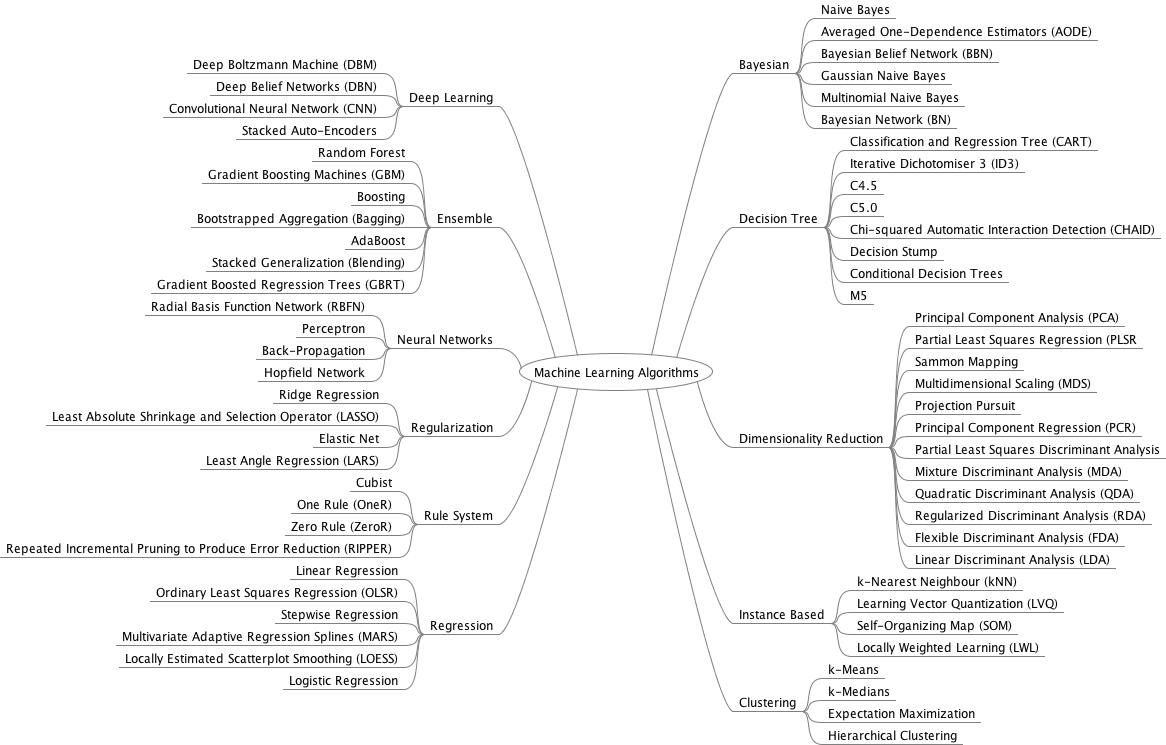
\includegraphics[height=14cm,width=16cm]{img/MLA.png}
  \caption{Jedno z možných členění \citep{mla}}
\end{figure}

\podsekce{Analýza vztahů}
Analýza vztahů, nebo také hledání asociačních pravidel. Je to metoda založená na pravidlech pro zjišťování zajímavých vztahů mezi proměnnými ve velkých databázích. Typickým příkladem dolování asociačních pravidel je tzv. analýza nákupního košíku (market
basket analysis). Tento proces analyzuje zvyky nakupujících a hledá závislosti mezi různým
zbožím, které si zákazníci vloží do svého nákupního košíku. Znalost informace o tom, které výrobky zákazníci obvykle kupují současně, mohou v praxi pomoci v tvorbě katalogů, pomáhají
při definování strategie rozmístění zboží v prodejně, ceny výrobků atd. \citep{burda}. Při získávání asociačních pravidel obvykle nemá vliv pořadí položek.
Typickými algoritmy pro tuto třídu je Apriori algoritmus, Eclat, FP-growth nebo třeba metoda GUHA, kterou objevili čeští vědci. 

\podsekce{Klasifikace a predikce}
Mezi klíčové části procesu dolování informací z databází patří klasifikace a predikce.
\paragraph{Klasifikace}
\leavevmode
\newline
Proces klasifikace je složen ze dvou kroků:
\begin{enumerate}
\item učení: tvorba klasifikačního modelu schopného klasifikovat data pomocí trénovacích dat
(vzorků dat u nichž známe výsledek klasifikace, neboli třídu, do které patří)
\item vlastní klasifikace: použití modelu pro klasifikaci nových dat (jejich zařazení do tříd\footnote{rozpad množiny záznamů do disjunktních tříd podle daného modelu klasifikace})
\end{enumerate}
\paragraph{Predikce}
\leavevmode
\newline
Jako predikce je označován proces určení dodatečných nebo chybějících hodnot
atributů analyzovaného záznamu. Jedním z druhů predikce je výše zmiňovaná vlastní klasifikace,
kdy se určuje dodatečný atribut představující třídu objektu (atribut diskrétního charakteru).
Jiným druhem predikce je regrese, kde jsou pomocí modelu vytvořeného klasifikací dopočítány
číselné hodnoty některého atributu spojitého charakteru.
\newline
Před samotnou klasifikací nebo predikcí je vhodné provést předzpracování dat (viz kapitola 4.2.6).

\podsekce{Umělé neuronové sítě}
Neuronové sítě  jsou výpočetní modely založené na zjednodušeném principu lidského mozku složeného z neuronů a synapsí. Nabývá formy v~podobě množiny vzájemně propojených jednotek (formálních neuronů). Jsou široce používané ve strojovém učení a rozeznávání vzorů \citep{bishop}. Každá vstupní proměnná odpovídá neuronu první úrovně zvané „vstupní vrstva“ a každá kategorie kvalitativní proměnné také odpovídá neuronu
ze vstupní proměnné. V některých případech, při použití sítě v~prediktivních metodách,
může existovat jedna nebo více závislých proměnných: každá z nich odpovídá jednomu
neuronu v konečné úrovni (výstupní vrstva). Prediktivní sítě spadají do skupiny
učení s učitelem a deskriptivní sítě spadají do učení bez učitele. 
\newline
\indent
Struktura neuronové sítě, zvaná také jako architektura nebo topologie, se skládá z počtu
vrstev neuronů, způsobů jak jsou jednotlivé neurony navzájem propojeny (výběr kombinačních
a přenosových funkcí) a~vah nestavitelných mechanismů. Volba struktury do
značné míry ovlivňuje výsledky, které budou získány. Nejdůležitější částí je implementace
neuronové sítě. Nejjednodušší strukturou je taková, ve které jsou neurony rozděleny
do dvou vrstev: do vstupní a výstupní vrstvy. Každý neuron ve vstupní vrstvě má
jeden vstup a jeden výstup, které se rovnají vstupu. Neuron přijme hodnoty
na svém vstupu a vrací $0$ až $n$ hodnot na výstupu. Všechny tyto hodnoty jsou normalizovány
tak, aby se vyskytovaly mezi hodnotou 0 až 1. Kombinační funkce spočítá první
hodnotu z propojených neuronů na vstupu a váhu připojení. Pro určení výstupní hodnoty se pro tuto hodnotu využívá přenosová funkce. Jednotky ve vstupní vrstvě jsou jednoduché ve smyslu, že nevytvářejí kombinace, ale pouze předávají
hodnoty proměnných. \citep{tuffery}
\newline
\indent
Stejně jako jiné metody strojového učení jsou neuronové sítě používány k řešení široké škály úloh, které by se jinak daly složitě řešit pomocí procedurálního nebo logického programování. Příkladem aplikace neuronové sítě je rozpoznávání ručně psaného písma nebo rozpoznávání hlasu.
\begin{figure}[!hbt]
  \centering
  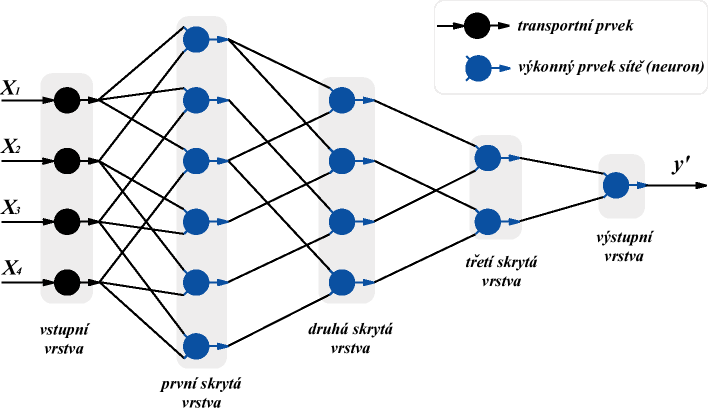
\includegraphics[scale=0.7]{img/struktura_site.png}
  \caption{Schéma neuronové sítě \citep{neuronobr}}
\end{figure}

\podsekce{SVM}
Mezi metody strojového učení s učitelem můžeme zařadit metodu Support vector machines (SVM). Slouží zejména pro klasifikaci a pro regresní analýzu. Na jejím vynalezení se podílel především ruský vědec Vladimir Vapnik.
Základem metody SVM je lineární klasifikátor rozdělující data do dvou tříd. Cílem úlohy je nalezení nadroviny, která prostor příznaků optimálně rozděluje tak, že trénovací data náležící rozdílným třídám leží v~opačných poloprostorech. Optimální nadrovina je pak taková, že hodnota minima vzdáleností bodů od roviny je co největší. Jinými slovy, okolo nadroviny je na obě strany co nejširší pruh bez bodů (maximální odstup, česky se tento pruh někdy nazývá také pásmo necitlivosti nebo hraniční pásmo). Na popis nadroviny stačí pouze body ležící na okraji tohoto pásma a těch je obvykle málo - tyto body se nazývají podpůrné vektory (support vectors) a odtud název metody.
\newline
\indent
Důležitou součástí techniky Support vector machines je jádrová transformace (kernel transformation) prostoru příznaků dat do prostoru transformovaných příznaků typicky vyšší dimenze. Tato jádrová transformace umožňuje převést původně lineárně neseparovatelnou úlohu na úlohu lineárně separovatelnou, na kterou lze dále aplikovat optimalizační algoritmus pro nalezení rozdělující nadroviny. Používají se různé kernelové transformace. 
Velkou výhodou této metody (a dalších metod založených na jádrové transformaci) je, že transformaci lze definovat pro různé typy objektů, nejen body v rovině. Např. pro grafy, stromy, posloupnosti DNA. \citep{schol}
\begin{figure}[!hbt]
  \centering
  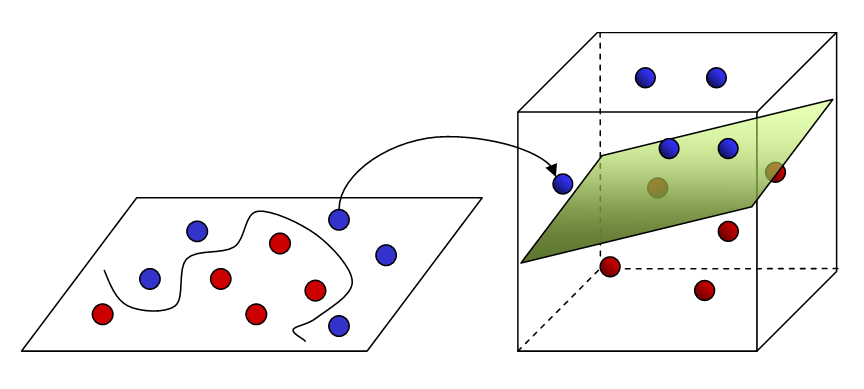
\includegraphics[scale=0.4]{img/svm.png}
  \caption{Transformace do vyšší dimenze}
\end{figure}

\podsekce{Shlukování}
Shlukování je typ strojového učení bez učitele. Jejím účelem je roztřídit
objekty do předem neznámých skupin (shluků) na základě podobnosti. O nově
vytvořených skupinách lze pak říci, že objekty v nich jsou si navzájem více
podobné, než objekty vně skupiny. Shlukování je vhodné pro analýzu velkého počtu
dokumentů, o kterých je předem známo málo informací. \citep{berry}
\newline
\indent
Pokud každý objekt patří právě do jedné skupiny, jedná se o pevné
shlukování (hard clustering). Druhým přístupem je měkké
shlukování (soft nebo fuzzy clustering), kdy jeden objekt může patřit
do více skupin. Jeho míra příslušnosti ke každé ze skupin pak může být vyjádřena hodnotou v intervalu <0;1>.
\newline
\indent
Typickou implementací shlukování je algoritmus k-Means. Ten na začátku
náhodně rozdělí objekty do $k$ shluků. Spočítá průměrný vektor pro každý
shluk (data jsou vyjádřena vektorovou reprezentací). Každý záznam pak
porovná s průměrným vektorem všech shluků. Poté přesune všechny objekty,
jejichž vektory byly blíže průměru jiného shluku než toho, ve kterém aktuálně jsou.
To se opakuje tak dlouho, dokud nepřestane docházet k přesunům. \citep{weiss}
\begin{figure}
  \centering
  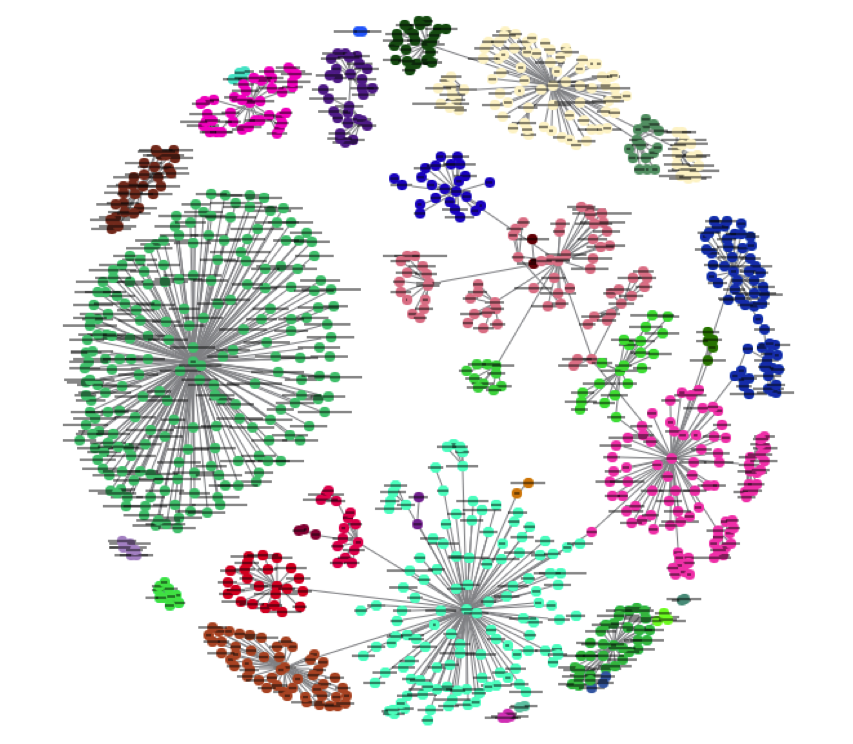
\includegraphics[scale=0.5]{img/clustering.png}
  \caption{Příklad shlukování \citep{clust}}
\end{figure}

\sekce{Dostupné datasety}
Pro testování jakýchkoliv data miningových algoritmů potřebujeme data, na kterých je možné algoritmy testovat. Na internetu je k nalezení množství veřejně dostupných datasetů. Namátkově několik z nich:
\begin{itemize}
\item http://tunedit.org/repo
\item http://repository.seasr.org/Datasets/UCI/arff/
\item http://www.kdnuggets.com/2011/02/free-public-datasets.html
\item http://archive.ics.uci.edu/ml/datasets.html
\item http://www.rdatamining.com/resources/data
\item https://github.com/fivethirtyeight/data
\item https://github.com/BuzzFeedNews
\end{itemize}
Datasetů můžeme najít libovolné množství. Problém však nastává, pokud potřebujeme najít pouze datasety s konkrétními atributy (např. jen numerické). Většina takto dostupných dat je posbírána z různých zdrojů (ať už firemní nebo lékařské záznamy, logy, sociální sítě) a v těchto databázích (datasetech) jsou atributy smíšených typů. Dalším problémem je nalezení podrobnějších informací o datech. Často je uvedeno odkud data pochází, ale co který atribut znamená už nikoliv. Extrémem jsou číselné datasety o kterých nemáme ani informaci o roku, kdy byla data sbírána, ani odkud pochází nebo co znamenají.
\newline
\indent
Tato diplomová práce se však nevěnuje specificky zaměřenému problému, proto nezáleží na původu dat ani na tom, kolik o nich je možné nalézt informací. Je ale potřeba, aby data měla určitou formu a pro konkrétní algoritmy i daný typ atributů. Použitým datasetům se věnuje kapitola 4.3 této diplomové práce.
 
\sekce{Výpočetní složitost algoritmů}
Při řešení programátorských úloh je vhodné mít nástroj, kterým lze porovnat efektivitu a rychlost provádění jednotlivých algoritmů. Pro tento účel byl zaveden pojem \textit{složitost algoritmu}.
\newline
\indent
Složitost algoritmu je kvalitativní charakteristikou algoritmu. Je to způsob klasifikace počítačových algoritmů. Určuje operační náročnost algoritmu tak, že sleduje, jak se bude chování algoritmu měnit v závislosti na změně velikosti nebo množství vstupních dat. Složitost slouží jako kritérium pro porovnávání kvality programů a algoritmů a ke zjištění jejich praktické použitelnosti.
\newline
\indent
Sledujeme časovou a prostorovou složitost. Časová složitost se odvíjí od počtu provedených operací. Prostorová složitost se odvíjí od velikosti datových struktur, které algoritmus využívá. Složitost se vyjadřuje jako matematická funkce, popisující závislost daného parametru (paměťového prostoru nebo spotřebovaného výpočetního času) na množství vstupních dat. \citep{rybicka}
\newline
\indent
Analýzou algoritmu můžeme skutečně vypočítat časovou složitost algoritmu, tj. čas potřebný pro provedení programu, ale pokud bereme v~úvahu všechny prováděné operace, je tento výpočet komplikovaný. Často, když hodnotíme efektivitu algoritmu, nepotřebujeme znát skutečnou časovou složitost, ale zajímá nás, jak rychle roste složitost v závislosti na rozsahu řešeného problému $n$. Např. zda lineárně nebo logaritmicky. Pak mluvíme o \textit{asymptotické} složitosti algoritmu a vyjadřujeme ji řádem růstu skutečné časové složitosti $T(n)$ nebo paměťové složitosti $S(n)$. \citep{hudec}
\newline
\indent
Složitost se obvykle zapisuje pomocí tzv. $O$-notace jako $O(f(N))$ - složitost je funkcí vstupních dat. Jde o \textit{třídu složitosti} a typ funkční závislosti, nikoli o přesné vyjádření.

\podsekce{Varianty složitosti}
Složitost závisí také na zpracovávaných datech a podle jejich charakteru se rozlišuje horní, dolní a střední (průměrný) odhad složitosti algoritmu.
\newline
\indent
\textbf{Horní odhad složitosti} algoritmu udává složitost algoritmu v nejhorším případě - algoritmus probíhá asymptoticky stejně rychle nebo rychleji než funkce $f(N)$. Nejčastěji se používá toto vyjádření, protože zahrnuje všechny, i ty nejhorší případy. Označuje se jako $O(f(N))$.
\newline
Definice $O$-notace:
\newline
Ať $f(n)$ a $g(n)$ jsou dvě nezáporné funkce definované na množině přirozených čísel $(N$). Říkáme, že $f(n)$ je velké $O$ od funkce $g(n)$ a zapisujeme $f(n) = O(g(n))$ nebo také $f(n) \in O(g(n))$, jestliže existuje přirozené číslo $n_0$ a konstanta $c > 0$ takové, že pro každé $n \geq n_0$ platí $f(n) \leq c \cdot g(n)$.
\newline
Ve zkratce:
\newline
$f(n) \in O(g(n)) \Leftrightarrow \exists n_0 > 0, \exists c > 0:\forall n \geq n_0: f(n) \leq c \cdot g(n)$
\newline
\indent
\textbf{Dolní odhad složitosti} udává ideální složitost algoritmu, která ovšem nastává jen pro určité případy vstupních dat. Označuje se jako $\Omega(f(N))$. Známe-li dolní odhad složitosti, je zřejmé, že danou úlohu nelze řešit efektivnějším algoritmem (který by spotřeboval méně času nebo prostoru). Algoritmus probíhá asymptoticky stejně rychle nebo pomaleji než funkce $f(N)$. Dokázat, že neexistuje lepší algoritmus, je ale těžší než odhadnout horní složitost.
\newline
Definice $\Omega$-notace:
\newline
Ať $f(n)$ a $g(n)$ jsou dvě nezáporné funkce definované na množině přirozených čísel $(N)$. Říkáme, že $f(n)$ je $\Omega$ od funkce $g(n)$ a zapisujeme $f(n) = \Omega(g(n))$ nebo také $f(n) \in \Omega(g(n))$, jestliže existuje přirozené číslo $n_0$ a konstanta $c > 0$ takové, že pro každé $n \geq n_0$ platí $f(n) \geq c \cdot g(n)$.
\newline
Ve zkratce:
\newline
$f(n) \in \Omega(g(n)) \Leftrightarrow \exists n_0 > 0, \exists c > 0:\forall n \geq n_0: f(n) \geq c \cdot g(n)$
\newline
\indent
\textbf{Průměrná (očekávaná) složitost} je střední hodnota složitosti při nějakém (náhodném) rozložení vstupních dat, algoritmus probíhá asymptoticky stejně rychle jako funkce $f(N)$. Označuje se jako $\Theta(f(N))$. Pokud algoritmus dosahuje horní složitosti jen zřídka, pak o složitosti algoritmu lépe vypovídá průměrná složitost.
\newline
Definice $\Theta$-notace:
\newline
Ať $f(n)$ a $g(n)$ jsou dvě nezáporné funkce definované na množině přirozených čísel $(N)$. Říkáme, že $f(n)$ je $\Theta$ od funkce $g(n)$ a zapisujeme $f(n) = \Theta(g(n))$ nebo také $f(n) \in \Theta(g(n))$, právě tehdy když současně platí $f(n) \in O(g(n))$ a $f(n) \in \Omega(g(n))$. Přesněji lze definici $\Theta-$notace přepsat pomocí přirozených konstant $c_1$ a $c_2$ následovně:
\newline
$f(n) \in \Theta(g(n)) \Leftrightarrow \exists c_1 > 0, \exists c_2 > 0, \exists n_0 > 0:\forall n \geq n_0: c_1 \cdot g(n) \leq f(n) \leq c_2 \cdot g(n)$ \citep{hanak}

\podsekce{Stanovení složitosti}
Stanovení složitosti algoritmu lze provést \textit{experimentálně} nebo \textit{analýzou zdrojového textu} algoritmu. Při experimentálním stanovení se měří spotřebovaný čas (prostor) pro vhodné hodnoty nezávisle proměnné. Stanovení provádíme tak, aby požadovaný charakter bylo možné interpolovat i~extrapolovat z tabulky získaných hodnot.
\newline
\indent
Při analýze zdrojového textu vyhledáváme cykly, jejichž počet opakování závisí na nezávisle proměnné (množství vstupních dat), a sledujeme těla takových cyklů.
\newline
\indent
Při stanovení časové složitosti nás zajímá počet operací, který je dán počtem opakování cyklu a implementační konstantou. Při vnoření cyklů se počty operací násobí. Stejně tak sledujeme rekurzivní volání - rekurze závislá na množství vstupních dat je ekvivalentní cyklu.
\newline
\indent
Stanovení prostorové složitosti znamená analýzu prostoru, který bude zabrán:
\begin{itemize}
\item pro statické proměnné (hledáme v deklaracích) - statické proměnné se obvykle na charakteru složitosti projeví jen konstantou,
\item pro dynamické proměnné (hledáme alokace paměti v příkazech, zejména v cyklech) - cyklické alokace jsou nejpodstatnější,
\item pro rekurzivně zabírané prostory (parametry volané hodnotou a lokální proměnné rekurzivních podprogramů) - podobně jako u cyklů hledáme počet rekurzivních zanoření v závislosti na množství vstupních dat.
\end{itemize}

\podsekce{Třídy složitosti}
Algoritmy můžeme rozdělit do tříd složitostí podle $O(N)$. Přitom platí, že algoritmus z vyšší třídy je pomalejší (prostorově náročnější) než algoritmus z předchozí třídy.
\newline
\indent
Pro malá $N$ nemusí být toto pravidlo zřetelné. Pokud ale patří dva algoritmy do různých tříd složitostí, pak vždy existuje takové množství dat, od kterého je asymptoticky lepší algoritmus (s nižší třídou složitosti) vždy efektivnější.
\newline
\indent
Konstanty, kterými se násobí funkce nebo se posunují vůči počátku souřadnic, nejsou vůbec podstatné. Není tedy důležité, jak rychlý počítač použijeme pro testování, není ani důležité, na jakém operačním systému a s jakými pomocnými prvky nebo přídavnými modifikacemi testovací úloha běžela. Často ani není možné efektivně určit kritické množství $n_k$, důležité je pouze zařadit algoritmus do dané třídy. \citep{rybicka}

\podsekce{Typické příklady časové složitosti algoritmů}
Konstantní složitost - $O(1)$
\begin{itemize}
\item indexování prvku v poli
\end{itemize}
Logaritmická složitost - $O(log N)$
\begin{itemize}
\item vyhledávání prvku v seřazeném poli metodou půlení intervalu
\item zařazení prvku do uspořádaného stromu
\end{itemize}
Lineární složitost - $O(N)$
\begin{itemize}
\item vyhledávání prvku v neseřazeném poli sekvenčním vyhledáváním
\item součet skupiny hodnot
\end{itemize}
Lineárně logaritmická složitost - $O(N \cdot logN)$
\begin{itemize}
\item řazení binárním uspořádaným stromem (průměrná složitost)
\item řazení hromadou, řazení slučováním
\end{itemize}
Kvadratická složitost - $O(N^2)$
\begin{itemize}
\item některé řadicí metody (Select sort, Insert sort...)
\item zpracování matice čísel (součet matic, nulování, transpozice), závislost je na řádu matice
\end{itemize}
Kubická složitost - $O(N^3)$
\begin{itemize}
\item násobení matic, závislost na řádu matic
\end{itemize}
Polynomiální složitost - $O(N^k)$
Exponenciální složitost - $O(k^N)$
\begin{itemize}
\item Přesné řešení problému obchodního cestujícího (v tomto případě $O(2^N)$)
\end{itemize}
Faktoriálová složitost - $O(N!)$
\newline
\newline

\noindent
Třídy jsou seřazeny vzestupně a platí:
\newline
$1 \ll log(N) \ll N \ll N \cdot log(N) \ll O(N^k) \ll  O(k^N) \ll O(N!)$

\podsekce{Prostorová složitost}
\textit{Prostorová složitost algoritmu} je počet registrů navštívených během výpočtu. Nepočítají se mezi ně registry obsahující vstup nebo výstup za předpokladu, že vstupní registry nelze přepisovat a do výstupních registrů lze psát jen výstup, který pak již rovněž nelze přepisovat. Proto mohou existovat algoritmy, které používají méně prostoru než je velikost jejich vstupu. Velikostí vstupu algoritmu je počet registrů, kde je vstup zapsán. Přitom předpokládáme, že čísla použitá k popisu vstupu se do registrů vejdou. Pokud by byla příliš velká, rozdělíme je do více registrů a práci s nimi zakódujeme do algoritmu. Délkou vstupu bude i v takovém případě počet použitých registrů. Stejným způsobem také ošetříme práci s~velkými čísly v průběhu algoritmu. Při práci s datovými strukturami považujeme za délku vstupu velikost reprezentované množiny.
\newline
\indent
Při výpočtu na skutečném počítači odpovídá prostorová složitost počtu bitů použitých programem během výpočtu. 
\newline
\indent
Obvykle se uvažuje jen prostorová složitost v nejhorším případě, i~když v datových strukturách, kde se různé reprezentace množiny mohou výrazně lišit, se vyšetřuje i očekávaná prostorová složitost. Amortizovaná prostorová složitost se ale nevyšetřuje. Častěji než očekávaná prostorová složitost se studují očekávané hodnoty nějaké kvantitativní charakteristiky použité reprezentace. Například to může být očekávaná výška binárních vyhledávacích stromů, které mají $n$ listů. \citep{koubek}

\podsekce{Snižování složitosti a efektivita algoritmů}
Složitost zvoleného algoritmu má přímý vliv na to, jak bude daný algoritmus efektivní. Nejčastěji je potřebné si uvědomit alespoň jednoduché případy, kdy při konstantní složitosti na množství vstupních dat nezáleží a čas potřebný pro zpracování je stále stejný, při lineární složitosti je spotřebovaný čas nebo prostor přímo úměrný množství dat a při kvadratické složitosti se při dvojnásobném vstupu zvýší potřeba času nebo prostoru čtyřikrát.
\newline
\indent
Cílem tedy je pracovat s algoritmy, které mají v nejhorším případě polynomiální složitost. Vyšší třídy (exponenciální, faktoriálová) jsou pro vyšší $N$ nepoužitelné a nepomohou ani rychlejší stroje. 
\newline
\indent
K nižší složitosti algoritmů přispívá jak optimální využití paměti, tak vhodná volba datových struktur - způsob uložení dat určuje i časovou a~paměťovou složitost práce s těmito daty, což může ovlivnit i výslednou složitost celého algoritmu.
\newline
\indent
Obě kritéria (čas, prostor) obvykle pracují proti sobě, proto si programátor musí zvolit, čemu dá přednost. V dnešní době se obvykle upřednostňuje zkrácení času. \citep{rybicka}

\kapitola{Algoritmy a jejich implementace}

\sekce{Výběr algoritmů a zdůvodnění}
Cílem této práce je výběr a testování algoritmů nejčastěji používaných pro data mining. Při výběru bylo primárně vycházeno z knihy \textit{The Top Ten Algorithms in Data Mining} a poté byl výběr přizpůsoben dalším kritériím a~použitému softwaru. Podle knihy \uv{The Top Ten Algorithms in Data Mining} je těchto deset nejpopulárnějších algoritmů: C4.5, k-Means, SVM,
Apriori, EM, PageRank, AdaBoost, kNN, Naive Bayes, CART \citep{top10}. Mezi další kritéria patřil například  výběr algoritmů z co nejvíce možných kategorií (klasifikace, regrese, pravidla, atd.). Proto byl například vynechán algoritmus CART, protože za zástupce klasifikačních stromových algoritmů už máme C4.5 a další. Algoritmus PageRank zase nemá žádnou implementaci v programu Weka, proto byl také nahrazen. 
\newline
\indent
Vybrané algoritmy byly následující: NaiveBayes, J48 (implementace C4.5), HoeffdingTree, SMO (trénovací algoritmus pro SVM), Apriori, SimpleKMeans (implementace k-Means), EM, IBk (implementace k-NN), LinearRegression, SimpleLogistic a JRip (implementace RIPPER). Algoritmy LinearRegression a SimpleLogistic byly přidány z důvodu pokrytí širšího spektra typů testovaných algoritmů (lineární a logistická regrese). Algoritmus JRip je jiným přístupem ke klasifikaci, založený na vyvozování pravidel. HoeffdingTree (implementace algoritmu VFDT) je pak zajímavým konkurentem algoritmu C4.5, přidán pro srovnání.  

\sekce{Použitý software}
Pro testování na reálných i syntetických datech bylo použito API programu Weka pro Javu. Samotný program Weka byl využit při generování syntetických dat. Weka je velmi vhodná pro testování algoritmů strojového učení jak z hlediska dostupnosti, tak z hlediska kvality a kvantity implementovaných algoritmů. Podle práce \uv{Porovnání nekomerčních nástrojů pro dolování znalosti z dat pomocí strojového učení} od Petra Ondrejky vyhrává program Weka i z hlediska časové náročnosti implementovaných algoritmů \citep{ondrejka}. Testování pak probíhalo v prostředí NetBeans IDE 8.2 s jazykem Java verze 8.

\sekce{Použitý hardware}
Pro účely této práce byl použit stolní počítač běžící na operačním systému Windows 10 Pro s touto konfigurací:
\begin{itemize}
\item Operační systém: Microsoft Windows 10 Pro 64-bit, verze 1709
\item Procesor: AMD Athlon(tm) II X4 631 Quad-Core 2.60 GHz
\item Operační paměť: 8GB DDR3
\item Základní deska: GigaByte GA-A75M-S2V
\item Pevný disk: WDC WD50000AAKB-00H8A0, 7200 ot./min., SATA, 500 GB
\end{itemize}

\sekce{Složitost algoritmů}
Tato sekce se věnuje popisu implementací použitých algoritmů a specifikuje jejich teoretickou složitost. Práce se omezuje pouze na srovnání horní meze teoretické složitosti, protože odhad dolní meze je pro zvolené algoritmy téměř nezjistitelný a pro účely práce nepodstatný. 

\podsekce{Klasifikace rozhodovacím stromem}
Jedním z typů klasifikačních modelů je rozhodovací strom. Rozhodovací strom může být
definován jako strom, kde každý nelistový uzel stromu představuje test na hodnotu atributu a
větve vedoucí z tohoto uzlu představují možné výsledky testu (např. test „muž nebo žena?“ a výsledky
„muž“ a „žena“). Listové uzly stromu jsou ohodnoceny identifikátory tříd (výsledky klasifikace).
\newline
\indent
Vlastní klasifikace rozhodovacím stromem probíhá cestou záznamu od kořene
stromu k jeho listu. V každém kroku prochází záznam testem v aktuálním uzlu rozhodovacího
stromu a dále pokračuje po větvi shodné s konkrétním výsledkem testu. Pokud takto
záznam dojde až do listového uzlu, je klasifikován třídou identifikovanou hodnotou příslušného
listu rozhodovacího stromu.
Z charakteru rozhodovacích stromů a~průběhu klasifikace je zřejmé, že pomocí rozhodovacích
stromů je možné provádět pouze predikci diskrétních hodnot (tedy vlastní klasifikaci) a
výsledky testů musí být diskrétního typu. Proto je nezbytné analyzovaná data spojitého charakteru
převést pomocí generalizace na data diskrétního charakteru\footnote{toto může být realizováno až při testu, například rozdělením výsledku testu atributu reálného typu na konečný počet intervalů}.\citep{rychly} 
\newline
\indent
Následuje popis zástupců této kategorie - algoritmu C4.5 a algoritmu Hoeffding Tree.
\paragraph{J48 (C4.5)}
Algoritmus J48 je ve skutečnosti algoritmus C4.8, jakožto 8. verze algoritmu C4.5, implementovaná v programu Weka. Časová složitost tohoto algoritmu je obecně $O(N m^2)$, kde $N$ je velikost trénovacích dat a $m$ je počet atributů. Podle tvůrce Weky, Dr. Eibe Franka, je však při aplikaci algoritmu na numerické atributy časová složitost vyšší. Aby bylo možné numerické atributy rovnoměrně rozdělit, je zde potřeba prohledat celý strom, což činí složitost této části $O(N^2)$. \citep{c45}
\paragraph{Hoeffding Tree}
Jedná se o rozhodovací strom s inkrementálním učením, který produkuje skoro identické
rozhodovací stromy jako tradiční dávkové algoritmy. Jako datovou strukturu používá Hoeffdingovy
stromy, založené na myšlence, že i malý vzorek dat může postačovat k výběru
optimálního dělícího atributu.
\newline
\indent 
Algoritmus Hoeffding tree používá Hoeffdingovu mez, aby s vysokou pravděpodobností
nalezl nejmenší počet $N$ vzorků, potřebných pro výběr dělícího atributu. Hoeffdingova mez
je nezávislá na pravděpodobnostní distribuci a měla by vybrat stejný dělící atribut jako při
použití nekonečného počtu vzorků. Hoeffdingovy stromy jsou nadále zkoumány, protože reprezentují jednu ze současných nejlepších technologií pro klasifikaci vysokorychlostních datových proudů. \citep{kirk}
\newline
\indent
Prostorová složitost VFDT (v programu Weka nese jméno HoeffdingTree) je $O(lmvq)$, kde $l$ je počet listů ve stromu, $m$ je počet atributů, $v$~je nejvyšší počet hodnot pro atribut a $q$ je počet tříd. Je tedy nezávislá na počtu instancí v~datasetu \citep{littman}. Časová složitost je pak $O(Nm)$. \citep{evag}

\podsekce{Klasifikace založená na pravidlech}
Rozhodovací (klasifikační) pravidla jsou lineárním zápisem rozhodovacích stromů.\footnote{avšak na rozhodovací pravidla lze převést také např. klasifikační model neuronové sítě \citep{han}}
Rozhodovací pravidla jsou složena z podmínky a závěru (if - then). Množina pravidel vzniká z rozhodovacího
stromu transformací, při které vyjádříme každou cestu z kořene do listu stromu jako
pravidlo, kde:
\begin{itemize}
\item podmínka pravidla je logický součin všech podmínek testů atributů (atribut = hodnota)
po cestě z kořene do listu,
\item závěr pravidla je klasifikace záznamu třídou v listu rozhodovacího stromu.
\end{itemize}
\indent
Samotná klasifikace probíhá na základě vyhodnocování rozhodovacích pravidel aplikovaných na analyzovaný záznam. Systém rozhodovacích pravidel obecně nestanovuje předem určené pořadí, které má být použito k vyhodnocování. Jinak je tomu u kombinovaných klasifikačních modelů (např. C4.5), kde každé pravidlo může být označeno hodnotou váhy, tedy jeho významnosti, a vyhodnocování souboru pravidel pak probíhá podle pořadí hodnot váhy v sestupném směru.
\newline
\indent
Další modifikací klasifikace pomocí systému rozhodovacích pravidel může být uplatnění \textit{fuzzy logiky},
kdy je příslušnost záznamu stanovena pro každou třídu hodnotou od 0 do 1, získanou aplikací
více pravidel. Každé úspěšné pravidlo přispěje ke klasifikaci záznamu do dané třídy.\footnote{typicky je výsledek pro třídu získán součtem všech pro ni úspěšných pravidel a~normalizací výsledku do intervalu <0,1>}
\newline
\indent
Klasifikační model založený na systému rozhodovacích pravidel lze zdokonalit využitím principů genetických
algoritmů. Je zřejmé, že každé pravidlo můžeme zakódovat do bitového řetězce určité délky
– např. očíslováním dílčích podmínek a převodem levé strany pravidla na řetězec bitů, kde bit
na n-té pozici reprezentuje přítomnost podmínky čísla n, a analogicky u pravé strany (očíslováním
tříd a řetězcem s pouze jediným kladným bitem). Pak můžeme provádět iterace a v každém
kroku provést dané operace genetických algoritmů: „crosover“ (vytvoření nového pravidla z levé a
pravé strany různých pravidel) a „mutation“ (inverzí náhodného bitu levé strany náhodně vybraného
pravidla). Po každé iteraci pak vyřadíme pravidla s velkou chybovostí na trénovacích datech. Pokud chybovost všech pravidel nepřekročí určené hranice, iterace končí a výsledkem je optimalizovaný systém rozhodovacích pravidel. \citep{rychly}
\newline
\indent 
Klasifikaci založenou na pravidlech implementuje (mimo jiných) algoritmus JRip.
\paragraph{JRip}
Algoritmus JRip (původní název RIPPER) byl implementován W. W. Cohenem v roce 1995. Zavedl do něj výrokové pravidlo RIPPER (Repeated Incremental Pruning to Produce Error Reduction) - tedy opakované přírůstkové prořezávání k redukci chyb. Cohen zavedl toto pravidlo kvůli zvýšení přesnosti pravidel nahrazením nebo opravou jednotlivých pravidel. Snižování chyby prořezáváním bylo používáno tam, kde bylo zapotřebí isolovat trénovací data a zastavit přidávání dalších podmínek k~pravidlu. Jako kritérium pro zastavení byla použita heuristika nazvaná \textit{délka minimálního popisu}. 
\newline
\indent 
Časová složitost tohoto algoritmu je $O(N log^2 N)$. \citep{ethem}

\podsekce{Regresní analýza}
Ve statickém modelování je regresní analýza statickým procesem pro odhad relací mezi proměnnými. Zahrnuje mnoho technik pro modelování a~analýzu několika proměnných, kdy je důraz kladen na vztah mezi závislou proměnnou a jednou nebo více nezávislými proměnnými (nebo „prediktory“). Regresní analýza pomáhá pochopit, jak se typická hodnota závislé proměnné mění, když se mění některá z nezávislých proměnných, zatímco ostatní nezávislé proměnné jsou udržovány fixní. Nejčastěji regresní analýza odhaduje podmíněné očekávání závislé proměnné vzhledem k nezávislým proměnným - tedy průměrné hodnotě závislé proměnné, pokud jsou nezávislé proměnné fixní. Méně často se zaměřuje na kvantilový nebo jiný parametr umístění podmíněného rozdělení závislé proměnné vzhledem k nezávislým proměnným. Ve všech případech je odhadovací cíl funkcí nezávislých proměnných nazývaných regresní funkce. V regresní analýze je také zajímavé charakterizovat variaci závislé proměnné kolem regresní funkce, která může být popsána rozložením pravděpodobnosti. \citep{freedman}
\paragraph{Linear Regression}
Časová složitost algoritmu Linear Regression je lineární, tedy $O(N)$. \citep{jordan}
\paragraph{Simple Logistic}
Algoritmus Simple Logistic je implementace logistické regrese v programu Weka. Časová složitost tohoto algoritmu je $O(N)$. \citep{jordan}

\podsekce{Bayesovské metody}
Naivní bayesovský klasifikátor je jednoduchý pravděpodobnostní klasifikátor, který vychází z Bayesova teorému. Bayesův teorém je platný pro diskrétní a kontinuální rozdělení pravděpodobností a je základním kamenem pro Bayesovskou statistiku. \citep{tuffery}
\newline
\indent
Základem naivního klasifikátoru je předpoklad, že jednotlivá pozorování $B_1, ..., B_n$ jsou podmíněně nezávislá při platnosti hypotézy $A$. Naivní - protože tento předpoklad je v úlohách reálného světa málokdy splněn. Je sice možné klasifikovat i neúplně popsané vzory, ale aposteriorní pravděpodobnost u chybějících vzorů v trénovací množině je nulová. 
\newline
\indent
Bayesovská síť je acyklický orientovaný graf, kde hrany představují závislosti mezi náhodnými veličinami a ke každému uzlu je přiřazena pravděpodobnostní distribuce ve tvaru \textit{P(uzel|rodič(uzel))}. Každý uzel je uspořádán a očíslován a každý jeho rodič má nižší pořadové číslo. Dále je každý uzel podmíněně nezávislý na všech uzlech s nižším pořadovým číslem s výjimkou svých rodičů a podmíněný rodičem rodičů. Vytvoření Bayesovské sítě se skládá ze dvou kroků:
\begin{itemize}
\item vytvoření struktury sítě
\item odhad pravděpodobnosti hodnot v tabulkách asociovaných s každým uzlem.
\end{itemize}
Výhodou Bayesovských sítí je možnost grafického znázornění znalostí. Výsledky jsou jednoduché pro lidskou interpretaci i modifikaci a mohou být využity k vykreslení závěrů. Závislosti mezi proměnnými mohou být
k vykreslení výsledků dokonce použity i tehdy, když některé proměnné nemohou být zkoumány. Dedukce tedy může vzniknout na základě nekompletních dat. \citep{tan}
\paragraph{Naive Bayes}
Časová složitost naivního bayesovského klasifikátoru je lineární, konkrétně $O(Nm)$, kde $N$ je počet instancí a $m$ je počet atributů. Paměťová složitost je $O(mqr)$, kde $m$ je počet atributů, $q$ je počet tříd a $r$~je průměrný počet hodnot pro atribut. \citep{chris}

\podsekce{Shlukování}
Ze shlukovacích algoritmů byl vybrán oblíbený K-Means a EM (Expectation Maximization). K-Means je nejjednodušší klasický shlukovací algoritmus, který je jednoduchý na implementaci. Může ovšem být použit jen pokud se veškerá data vejdou do paměti. Jméno dostal podle toho, že každý z $k$ shluků je reprezentován průměrem (mean) objektů v něm.
\newline
\indent
Na rozdíl od K-Means, metoda EM je založena na předpokladu, že objekty v datasetu mají hodnoty rozdělené podle nějaké (neznámé) lineární kombinace jednoduchého rozdělení pravděpodobnosti. Zatímco K-Means přiřazuje objekty do shluků s cílem minimalizovat variaci uvnitř skupiny, EM přiřazuje objekty do rozdílných shluků s určitými pravděpodobnostmi za účelem maximalizovat pravděpodobnost přiřazení. Jinými slovy, přiřazuje každý objekt do shluku podle jeho pravděpodobnosti členství. Nejsou zde žádné striktní hranice mezi shluky. \citep{uddin}
\paragraph{K-Means}
Prostorová (paměťová) složitost tohoto algoritmu je $O((N+k)m)$, kde $N$ je počet instancí a $m$ je počet atributů. Časová složitost je pak $O(tkNm)$, kde $t$ je počet iterací potřebných pro konvergenci. $t$ je často malé a může být vázáno, protože většina změn se typicky děje v prvních pár iteracích. Je tedy lineární vzhledem k $N$, a jednoduchý a efektivní v~případě, že počet shluků $k$ je značně menší než $N$.   
\paragraph{EM}
Časová složitost je zde lineární vzhledem k počtu instancí, atributů a~iterací. $O(Nmt)$, kde $t$ je počet iterací. \citep{uddin}

\podsekce{Algoritmy líného učení}
Algoritmy líného učení nebo také učení založené na instancích (instance-based learning) můžeme obecně rozdělit na \uv{líné učení} (lazy learning) a \uv{dychtivé učení}  (eager learning).  Algoritmy líného učení uchovávají v~paměti všechna trénovací data a čekají na vstup testovacích dat. Poté vyhledávají v trénovacích datech instanci, která nejvíce odpovídá nové (testovací) instanci a podle toho ji klasifikuje. Výhody tohoto přístupu jsou v tom, že data nejsou ovlivněna předešlými výpočty a data se velmi snadno aktualizují. Nevýhodami může být možná velikost paměti potřebné k uchování dat a tím pádem i pomalejší klasifikace (při klasifikaci nové instance je vždy nutné začít prohledávat od začátku, přes všechna uložená trénovací data), nebo potřeba velmi dobře zvolit parametry a~nastavení algoritmu, aby ukazoval správné výsledky.
\newline
\indent
Algoritmy dychtivého učení se liší v tom, že kompilují trénovací data do modelu nebo zhuštěného popisu a pak trénovací data zahodí. Klasifikace nových instancí pak probíhá na základě vytvořeného modelu. To umožňuje dosáhnout lepšího času při predikci, ale na rozdíl od líného učení musíme provést i tréning dat. Patří mezi ně algoritmy jako  IB1 až IB3, k-NN, rozhodovací stromy, SVM.
\paragraph{IBk (k-NN)}
Nejznámější algoritmus učení založeného na instancích je k-NN ($k$ nejbližších sousedů - $k$ Nearest Neighbor). Ten nahlíží na každý objekt jako součást n-dimenzionálního prostoru, kde $n$ je počet atributů. Poté počítá standardní Euklidovskou vzdálenost mezi novou testovací instancí a ostatními instancemi v trénovací množině. Klasifikace je pak určena pomocí $k$ nejbližších sousedů. 
\newline
\indent
Časová složitost algoritmu IBk je kvadratická,  $O(N^2)$. \citep{oniev}
\paragraph{SMO (SVM)}
SMO je implementace trénovacího algoritmu pomocných vektorů (SVM) v programu Weka. Podle Pedra Domingose se algoritmus SVM se také řadí mezi algoritmy založené na instancích \citep{pedro}. Důvodem je mimo jiné nutnost uložení pomocných vektorů v paměti. Časová složitost lineárního SVM je lineární, vzhledem k počtu pomocných vektorů \citep{oli}. Časová složitost nelineárního SVM je pak mezi $O(N^2)$ a $O(N^3)$ \citep{lin}. Paměťová složitost SMO je $O(N^2)$. \citep{zeng}

\podsekce{Asociační pravidla}
Celkový počet pravidel, které lze vytěžit z datasetu s $c$ atributy je $3^c - 2^{c+1} + 1$. Běžnou strategií využívanou v algoritmech pro hledání asociačních pravidel je rozklad problému do dvou dílčích úkolů - generování frekventovaných vzorů a generování asociačních pravidel. Úkolem generování frekventovaných vzorů je nalezení predikátů, které mají podporu vyšší, než je zadaná minimální hodnota (nalezení silných množin). Generování asociačních pravidel využívá silných množin a odstraňuje pravidla, jejichž spolehlivost nedosahuje předem určené minimální hodnoty. Výpočetní nároky pro generování frekventovaných vzorů jsou obecně vyšší než ty pro generování asociačních pravidel. Dataset s $c$ atributy může vygenerovat až $2^c-1$ frekventovaných vzorů. Hledání frekventovaných vzorů metodou \uv{hrubé síly} - tedy porovnání každého kandidáta s každou transakcí je $O(N M w)$, kde $N$ je počet transakcí, $M=2^c-1$ a $w$ je maximální šířka transakce. Časová složitost pro generování asociačních pravidel roste lineárně s velikostí datasetu. \citep{tan}
\paragraph{Apriori}
Podle výzkumu Markuse Heglanda je časová složitost Apriori algoritmu obecně $O(Nm^2)$, kde $N$ je počet instancí a $m$ je počet atributů. Tato složitost jde snížit až na $O(Nm)$ použitím vhodných datasetů. \citep{hegland}

\kapitola{Praktická část}

\sekce{Porovnání teoretické složitosti algoritmů}
Teoretické složitosti vybraných algoritmů se samozřejmě velmi liší. Složitost závisí jak na typu algoritmu, tak na jeho implementaci, způsobu řešení problému, nastavení parametrů i na vstupních datech. U některých algoritmů se složitost určuje obtížně, protože o nich buď zatím není dostatek informací a nebo by pro zjištění horní hranice na velkých N bylo zapotřebí neúměrně mnoho času. Obecné složitosti vybraných algoritmů jsou shrnuty v kapitole 4.1.2. 

\podsekce{Teoretická prostorová složitost}
Prostorová složitost algoritmu může být definována jako celkové množství paměti potřebné pro jeho výpočet. Pro výpočet programu je obecně zapotřebí počítačová paměť ze tří důvodů:
\begin{itemize}
\item Prostor pro instrukce: Paměť potřebná pro uložení zkompilované verze instrukcí
\item Environmentální zásobník: Paměť pro uložení částí výpočtu
\item Datový prostor: Paměť pro uložení všech konstant a proměnných
\end{itemize}
Při provádění analýzy prostorové složitosti algoritmu ovšem uvažujeme pouze datový prostor - tedy paměť potřebnou pro uložení struktur, konstant a proměnných. Prostor pro instrukce i environmentální zásobník ignorujeme. Na to, abychom mohli úspěšně provést analýzu prostorové složitosti algoritmu, potřebujeme znát přesné množství paměti využité pro uložení různých hodnot datových typů. Toto množství je závislé na překladači. 
\newline
\indent
Zjištění teoretické složitosti vybraných algoritmů je však velmi obtížný úkol. Obecně to lze provést dvěma způsoby: analýzou kódu algoritmu nebo experimentálně (viz kapitola 2.6.2). 
\newline
\indent
Analýza kódu zde není možná, protože implementační kód algoritmů není ve většině případů dostupný. I kdyby byl, toto téma by nejspíše odpovídalo obsahu několika diplomových prací. Bohužel, ani autoři těchto implementací ve svých publikacích většinou neuvádí teoretickou prostorovou složitost. Je to buď z důvodu obtížnosti analýzy a nebo přisuzování menšího významu vzhledem k časové složitosti.
\newline
\indent
Odhad prostorové složitosti použitím úměrného množství testů se jeví jako přijatelnější možnost. Tato možnost je preferovaná autory implementací použitých algoritmů, pokud se prostorovou složitostí vůbec zabývají. Odhadnout prostorovou složitost všech zvolených algoritmů by byl na základě provedených testů realizovatelný úkol, avšak výrazně nad rámec obsahu práce (bylo by také nutné provést větší množství testů). V přiložených tabulkách jsou podklady pro budoucí analýzu. Tato práce se v~dalších odstavcích zabývá především časovou složitostí s několika výjimkami ukázek prostorové složitosti u algoritmů, které mají tuto informaci dostupnou z publikací od autorů dané implementace. 
\newline
\newline
\begin{tabular}{c||rp{3cm}}
    \bfseries \bfseries Algoritmus & \bfseries Prostorová složitost \\[2mm]
    \hline \hline
    HoeffdingTree (VFDT) & $O(lmvq)$ \\
    Naive Bayes & $O(mqr)$ \\
    K-Means & $O((N+k)m)$ \\
    EM & $O(Nmt)$ \\
    SMO (SVM) & $O(N^2)$ \\
    \end{tabular}
\newline
\newline
$N$ udává počet instancí, $m$ počet atributů, $t$ je počet iterací, $q$ je počet tříd, $r$ je průměrný počet hodnot pro atribut, $l$ je počet listů ve stromu, $k$~je počet shluků pro K-Means. 
\newline
\newline
Je zřejmé, že přehledné a snadno čitelné vyobrazení těchto složitostí je nemožné. Pro zobrazení 3 proměnných bychom potřebovali 3D prostor a~zobrazení 4 a více proměnných už není možné na papír vykreslit. Částečně si můžeme pomoct vhodnými vstupními daty - stejný počet atributů, tříd. 

\podsekce{Teoretická časová složitost}
Obecné složitosti vybraných algoritmů jsou shrnuty v kapitole 3.4, zde je pro přehlednost uvedena tabulka časových složitostí.
\newline
\newline
\begin{tabular}{c||rp{3cm}}
    \bfseries \bfseries Algoritmus & \bfseries Časová složitost \\[2mm]
    \hline \hline
    J48 (C4.5) & $O(Nm^2)$ až $O(N^2)$ \\
    HoeffdingTree (VFDT) & $O(Nm)$ \\
    JRip & $O(N log^2 N)$ \\
    Linear Regression & $O(N)$ \\
    Simple Logistic & $O(N)$ \\
    Naive Bayes & $O(Nm)$ \\
    K-Means & $O(tkNm)$ \\
    EM & $O(Nmt)$ \\
    IBk (k-NN) & $O(N^2)$ \\
    SMO (SVM) & $O(N^2)$ až $O(N^3)$ \\
    Apriori &$O(Nm)$ až $O(Nm^2)$ \\
    \end{tabular}
\newline
\newline
$N$ udává počet instancí, $m$ počet atributů, $t$ je počet iterací, $k$ je počet shluků pro K-Means. 

\sekce{Metodika}
Součástí této práce bylo vyhledání a využití datasetů s reálnými daty pro testování algoritmů. Zde ovšem nastává problém zmíněný v kapitole 2.5. Nejenže je často obtížné zjistit původ a detailní informace o datech, ale mnohdy ani nemáme možnost určit jejich význam. Pro testování na reálných datech byly pro účely této práce vybírány reálné datasety z důvěryhodných internetových zdrojů (např. UCI repository, StatLib, Hawlett-Packard Labs), ale i zde můžeme občas narazit na zmíněné problémy. Cílem této práce však není zjišťování informací a vztahů z konkrétních dat, proto můžeme význam i informace o těchto datech zanedbat. Kapitola 4.3 se blíže věnuje použitým datasetům a obsahuje o nich základní informace.
\newline
\indent
Testování algoritmu probíhá obyčejně tak, že se algoritmus natrénuje na trénovacích datech a poté se otestuje na datech testovacích. Tréning algoritmu nám udává s jakou chybou můžeme pak počítat u testovacích dat. V této práci nás ovšem přesnost algoritmu nezajímá, proto zde ani tyto výsledky nejsou uvedeny.\footnote{součástí práce je přiložené CD a na něm jsou uvedeny výsledky testování včetně přesnosti algoritmů, počtu nalezených shluků, počtu nalezených pravidel a další zajímavé údaje} Bylo ale zapotřebí provést i tréning i testing, protože tyto kroky jsou součástí každého dolování z dat a cílem této práce je ukázat reálné výsledky časové a paměťové složitosti při běžném využití algoritmů pro data mining. Použité reálné datasety nedělí svůj obsah na trénovací a testovací část, proto byla při testování použita crossvalidace. Způsob trénování a testování crossvalidací je obecně nejběžnějším způsobem při práci s data miningovými algoritmy. Měření pro každý dataset bylo 5x opakováno, aby byly splněny základní statistické požadavky a eliminovány náhodné vlivy. 

\podsekce{Java virtual machine}
Pro samotné testování na datech si Java (konkrétně JVM - Java Virtual Machine) automaticky alokuje potřebnou operační paměť. Má však různá výchozí nastavení s maximálními limity, aby některé části výpočtu nezabraly veškerou paměť a tím by se běh zastavil s chybou. Veškeré vytvořené objekty se ukládají do haldy, jejíž velikost závisí na velikosti objektů. Takto se může halda rozpínat dokud nedosáhne svého nastaveného maxima (nebo limit operační paměti). Bohužel ve výchozím nastavení je maximum paměti pro velikost haldy (heap space) nastaveno na pouhých ~64 MB, což je pro testování na velkých datasetech naprosto nevhodné. Toto nastavení lze změnit příkazem -Xmx určujícím maximální velikost haldy při běhu. V předešlých verzích Javy bylo pro změnu velikosti využívané paměti potřeba pracovat i s parametrem -Xms (úvodní nastavení velikosti haldy). Tento parametr byl ovšem odstraněn ve verzi Java 8 (nahrazen třídou Metaspace\footnote{https://dzone.com/articles/java-8-permgen-metaspace}).  
\newline
\indent
Pro potřeby této práce byla velikost haldy (a tím pádem velikost využitelného prostoru pro struktury algoritmů) nastavena na 8 GB, což umožňovalo i běh algoritmů náročnějších na velikost operační paměti. 

\podsekce{Velikost operační paměti potřebné pro běh algoritmu}
Sledovat velikost operační paměti potřebné pro běh algoritmů na různých datasetech můžeme v Javě několika způsoby. Podle blogu Philippe Fournier-Vigera\footnote{http://data-mining.philippe-fournier-viger.com/how-to-measure-the-memory-usage-of-data-mining-algorithms-in-java/} jsou nejlépe využitelné dva způsoby. Prvním je měření operační paměti spotřebované při běhu celého programu. To ovšem naráží na zásadní problém a tím je fakt, že v Javě nemá programátor možnost kontrolovat alokaci operační paměti pro běh programu. O to se stará JVM automaticky. Java využívá tzv. Garbage Collector pro uvolnění paměti a ten je stavěn na \uv{líném} přístupu. Jinými slovy, nikde není zaručeno, že Garbage Collector okamžitě uvolní již nevyužívanou část paměti. Dokonce občas při nadměrné práci procesoru nechává paměť záměrně naplnit až do svého maxima a až poté začne s uvolňováním. To ovšem zpomalí rychlost běhu algoritmu a může tím pádem vést k nepřesným výsledkům jak z hlediska času, tak z hlediska využití operační paměti. 
\newline
\indent
Druhým způsobem je měření velikosti paměti využité třídou Java Object. Programovací jazyk Java je objektový jazyk a tím pádem i veškeré algoritmy a datové struktury tvořené těmito algoritmy jsou také objekty. Proto můžeme snadno přistoupit k datové struktuře vytvořené jakýmkoliv algoritmem pro svůj výpočet a změřit její velikost, kterou zabírá v~operační paměti. Tento způsob je mnohem přesnější než první. Je také jediný použitelný při porovnávání naměřených výsledků s teoretickou funkcí prostorové složitosti, protože ta hovoří pouze o paměti zabrané vytvořenou strukturou algoritmu. 
\newline
\indent
Velikost operační paměti na stroji použitém pro testování byla 8 GB, což dávalo prostor pro běh všech algoritmů na téměř všech velkých datasetech bez problému s dosažením maxima operační paměti a tedy ovlivněním výsledků testování. V níže uvedených grafech je znázorněn druhý způsob sledování paměti (tedy velikost operační paměti využité pro uložení datové struktury), nicméně v přiložených tabulkách je uvedena i celková paměť potřebná pro běh algoritmu. Pro účely této práce byly tedy využity oba způsoby měření operační paměti. Údaj o celkové paměti může ulehčit rozhodování volby algoritmu a jeho implementaci v případě použití stroje s omezenou RAM pamětí. 

\podsekce{Knihovna weka a jdmp}
Pro běh algoritmů v prostředí NetBeans byly využity knihovny Weka a~jdmp\footnote{https://jdmp.org/}. Knihovna Weka (nebo také Weka api) je rozhraní vytvořené pro javu universitou Waikato, stejně jako celý program Weka s uživatelským rozhraním. Toto rozhraní slouží pro využití implementovaných algoritmů s vlastním kódem. Program Weka například neumožňuje zobrazit operační paměť potřebnou pro běh algoritmu, což ovšem lze sledovat odlišnými způsoby při využití jazyka Java a JVM. 
\newline
\indent
Knihovna jdmp je velmi vhodná pro vlastní testování, protože v sobě zahrnuje nejen Weka api, ale i další knihovny a implementace algoritmů, které ve Weka api chybí. Navíc automaticky počítá čas běhu programu s~ohledem na tisíciny sekundy. 

\podsekce{Předzpracování dat}
Předzpracování dat (preprocessing) je důležitou součástí data miningu. Datasety mnohdy obsahují chybné hodnoty dat, chybějící nebo duplicitní údaje i neplatné datové kombinace. Bez preprocessingu by tato data mohla způsobovat chybné nebo zavádějící výsledky. Příprava dat a jejich filtrování se obecně skládá z těchto kroků:
\begin{itemize}
\item čištění dat – odstraňuje šum, případně snižuje jeho míru a doplňuje chybějící hodnoty (např. s
využitím regresní analýzy)
\item určení relevance dat – jsou odstraněna irelevantní a redundantní data, případně jsou záznamy
ohodnoceny vahou jejich významu
\item transformace dat – zahrnuje generalizaci\footnote{především za účelem převedení spojitých typů atributů na diskrétní typy, které jsou lépe použitelné v některých typech
klasifikačních modelů}
a normalizaci dat\footnote{normalizovaná data jsou výhodná např. pro neuronové sítě} za účelem přizpůsobení použitému klasifikačnímu modelu \citep{rychly}
\end{itemize}

Datasety vybrané pro tuto práci byly z převážné části již předzpracované, tudíž nebyla potřeba tyto kroky znovu opakovat. Jediná podstatnější úprava na datech byla provedena při uzpůsobování datasetů pro algoritmus Apriori (ten za vstup musí mít pouze nominální atributy) a~převod .csv souborů datasetů do .arff souborů, vhodných pro Weku. 

\podsekce{Zobrazení výsledků}
Délka výpočtu algoritmu i místo v paměti zabrané pro jeho výpočet závisí z největší části na vstupu dat. Nejvýznamnější faktor pro vstupní dataset je počet jeho instancí. Od toho se také odvíjí velikost datasetu. Následuje počet atributů datasetu a ostatní faktory jako je počet tříd, pravidel, shluků... Čas výpočtu a paměťového prostoru zabraného algoritmem dále závisí také na počtu iterací potřebných pro výpočet a celkovém nastavení parametrů použitého algoritmu.
\newline
\indent
Nejvhodnější způsob znázornění výsledků této práce je nejspíše grafickou formou, nejlépe 2D grafem. Zde však opět narážíme na překážku zmíněnou v kapitole 4.2.5. Čitelné zobrazení více než dvou proměnných je možné pouze ve vícerozměrných prostorech. Použitím papíru jsme omezeni na zobrazení maximálně tří dimenzí, ale i 3D model chování algoritmu na datasetu (např. závislost času na počtu instancí a atributů) by byl v mnoha případech obtížně čitelný. 
\newline
\indent
Časová složitost vybraných algoritmů je většinou závislá na dvou proměnných (počtu instancí a počtu atributů). V případě testování na uměle vytvořených datech si můžeme pomoct tím, že jednu nebo více proměnných zvolíme jako konstantu (např. všechny vstupy budou mít stejný počet atributů). Díky tomu je možné zobrazit časovou závislost na počtu instancí grafem. V případě testování na reálných datech si však takto pomoct nemůžeme, protože tato data jsou velmi různorodá. Vyobrazení chování algoritmu na reálných datech v případě zanedbání jedné z proměnných je potom nesmyslné. V následujících částech práce se proto omezíme na grafické znázornění chování algoritmů na syntetických datech a jeho porovnání s teoretickou časovou složitostí. Kompletní výsledky testů na všech datech jsou pak uvedeny v přiložených tabulkách.

\podsekce{Teoretická křivka složitosti}
Teoretická křivka časové i paměťové složitosti byla pro potřeby grafického znázornění získána interpolací vzhledem k funkci složitosti. Následná uvedená zobrazení této křivky nemusí být dokonale přesná, ale dávají nám možnost porovnat mezi sebou reálně naměřené hodnoty s~hodnotami teoretickými. 

\podsekce{Porovnání výsledků}
Pro porovnání naměřených hodnot s jejich teoretickým předpokladem se jeví grafické znázornění jako nejsrozumitelnější možnost. Z uvedených grafů můžeme snadno vyčíst, jestli se reálná náročnost opravdu blíží teoretické a nebo jestli je horní odhad složitosti vysoce nadsazen pro běžné použití algoritmu. 
\newline
\indent
Mezi sebou můžeme srovnat pouze algoritmy určené pro stejnou úlohu, nejlépe spuštěné na stejných vstupech. Pro tuto práci byly vybrány algoritmy na základě jejich oblíbenosti používání v data miningu a~jsou tedy určeny pro různé úlohy. Srovnání všech algoritmů mezi sebou je proto nemožné. Kapitola 6 se věnuje částečnému porovnání vybraných algoritmů pro stejnou úlohu.

\sekce{Použité datasety}
Jak již bylo zmíněno, reálné datasety použité pro testování algoritmů byly získány z různých zdrojů. Mezi hlavní patří sbírky získané z UCI repository, StatLib a Hawlett-Packard Labs\footnote{Vše dostupné z https://weka.wikispaces.com/Datasets}. Následující tabulky uvádí pro zajímavost základní informace o některých použitých datasetech.\footnote{Kompletní soubor použitých datasetů spolu s tabulkou informací se nachází na přiloženém CD}

\podsekce{Generování dat}
Program Weka má k dispozici několik generátorů dat pro různé druhy úloh. Každý generátor má další volitelná nastavení, aby vygenerovaný dataset odpovídal veškerým požadavkům. Nastavení generátorů, stejně jako nastavení algoritmů, je popsáno v kapitole 5. Datasety nebyly rozděleny na trénovací a testovací, pro ohodnocení použita crossvalidace (stejně jako u reálných datasetů). 

\podsekce{Tabulka reálných datasetů}
\begin{table}[h]
\begin{tabular}{  p{4.4cm}  p{1.9cm}  p{3.5cm}  p{3.5cm}  }

{\bf název} &  {\bf typ} & {\bf počet instancí} & {\bf počet atributů} \\

new3s.wc &      numeric &       9558 &      26833 \\

ohscal.wc &     numeric &      11162 &      11466  \\

la1s.wc &    numeric &       3204 &      13196 \\

Data\_Cortex\_Nuclear &      nominal &       1080 &         82  \\

mfeat-karhunen &      numeric &       2000 &         65 \\

nursery &       nominal &      12960 &          9  \\

optdigits &   numeric &       5620 &         65 \\

letter &  numeric &      20000 &         17 \\

75000i &    nominal &     266209 &          3  \\

\end{tabular}
\end{table} 

\newpage
\podsekce{Tabulka generovaných datasetů}
\begin{table}[h]
\begin{tabular}{  p{4.4cm}  p{1.9cm}  p{3.5cm}  p{3.5cm}  }
{\bf název} &  {\bf typ} & {\bf počet instancí} & {\bf počet atributů} \\

200000-100-class &      nominal &                 200000 &        100 \\

10000-50-class &       nominal &                  10000 &         50 \\

5000-30 &          nominal &                   1000 &         10 \\

400000-reg &      numeric &                 400000 &          2 \\

100000-reg &       numeric &                 100000 &          2 \\

160000-100-clust &     numeric &                 160000 &        100 \\

200000-100-rul &      numeric &                 200000 &        100 \\

1000-10-rul &          numeric &                   1000 &         10 \\
\end{tabular}
\end{table}  

\kapitola{Výsledky experimentů}
Pro uvedená zobrazení a jejich popis platí stejná legenda jako v ostatních částech práce. $N$ udává počet instancí, $m$ počet atributů, $t$ je počet iterací, $q$ je počet tříd, $r$ je průměrný počet hodnot pro atribut, $l$ je počet listů ve stromu, $k$ je počet shluků pro K-Means. 
\newline
\indent
Oranžová křivka je křivkou naměřených hodnot, modrá křivka znázorňuje teoretické hodnoty podle funkce složitosti. Ve většině případů je vodorovná osa v logaritmických hodnotách, pro přehlednější zobrazení výsledků na všech velikostech testovaných datasetů.
\newline
\indent
U nastavení generátorů a implementací algoritmů se omezíme na částečný výčet podstatných parametrů a jejich hodnot. Podrobnější popis významu jednotlivých parametrů je dostupný v programu Weka, nebo v~dokumentaci implementace algoritmu.\footnote{http://weka.sourceforge.net/doc.dev/}

\newpage
\sekce{NaiveBayes}
\paragraph{Charakter vstupních dat}
Data pro 10 vstupních datasetů byla generována pomocí BayesNet generátoru. Parametr \textit{cardinality} (počet tříd) byl nastaven 2, počet atributů 30 s nominálními hodnotami, počet instancí od 1000 po 300000.\footnote{Při zvolení vyššího počtu instancí se program Weka zasekl a následně spadl.} Průměrný počet hodnot pro atribut $r$ i počet tříd $q$ zde považujeme za konstanty, proto je možné zobrazení časové i paměťové závislosti na počtu instancí.
\paragraph{Nastavení algoritmu}
Nastavení implementace bylo ponecháno na výchozích hodnotách Weky.
\begin{figure}[hbp]
  \centering
  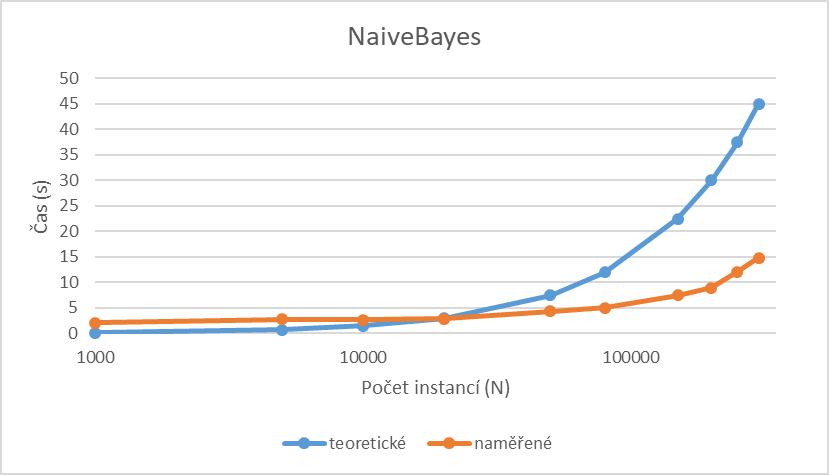
\includegraphics[scale=1]{img/nb.png}
  \caption{NaiveBayes - čas v závislosti na počtu instancí}
\end{figure}
\podsekce{Čas}
Teoretická časová složitost této implementace je $O(Nm)$. Z obrázku 5 lze vyvodit, že lineární složitost je pro běžná použití nadsazená a průměrný čas měření by mohl spadat do nižší kategorie složitosti. 
\podsekce{Paměť}
Obecná paměťová složitost algoritmu Naive Bayes je $O(mqr)$, podle práce \textit{A naive Bayes classifier on 1998 KDD Cup} \citep{chris}. Je tedy nezávislá na počtu instancí. V programu Weka tomuto typu odpovídá implementace \textit{NaiveBayesUpdateable}, který použije výchozí přesnost 0,1 pro číselné atributy, když je classClassifier volán s nulovými trénovacími instancemi. V této práci byla však zkoumána jiná implementace (\textit{NaiveBayes}), která na počtu instancí závislá je, jak vyplývá z obrázku 6. Teoretická prostorová složitost této implementace nebyla zjištěna, ale podle vývoje v grafu můžeme odhadovat, že se nachází v kategorii lineární složitosti, nejspíš $O(Nm)$.
\begin{figure}[hbp]
  \centering
  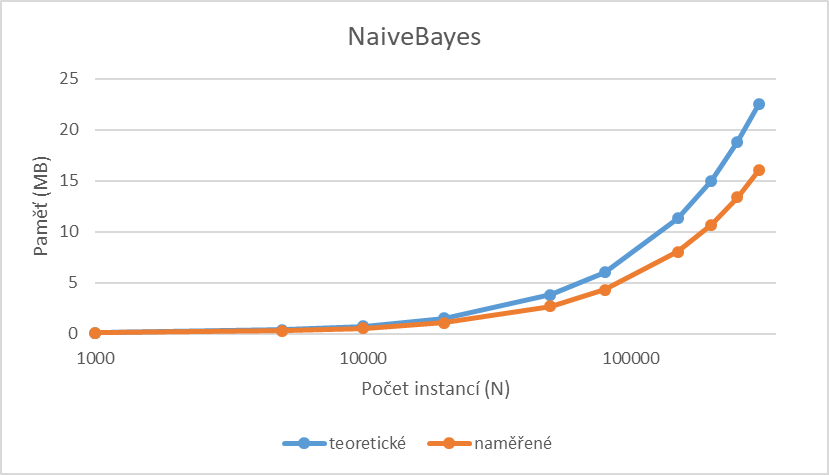
\includegraphics[scale=1]{img/nbp.png}
  \caption{NaiveBayes - paměť v závislosti na počtu instancí}
\end{figure}

\newpage
\sekce{J48}
\paragraph{Charakter vstupních dat}
Pro běh algoritmu byla použita stejná vstupní data jako pro NaiveBayes.
\paragraph{Nastavení algoritmu}
Parametr \textit{confidenceFactor} byl nastaven na 0,25, \textit{minNumObj} (minimální počet instancí pro list) 2, \textit{numFolds} 3. 
\begin{figure}[hbp]
  \centering
  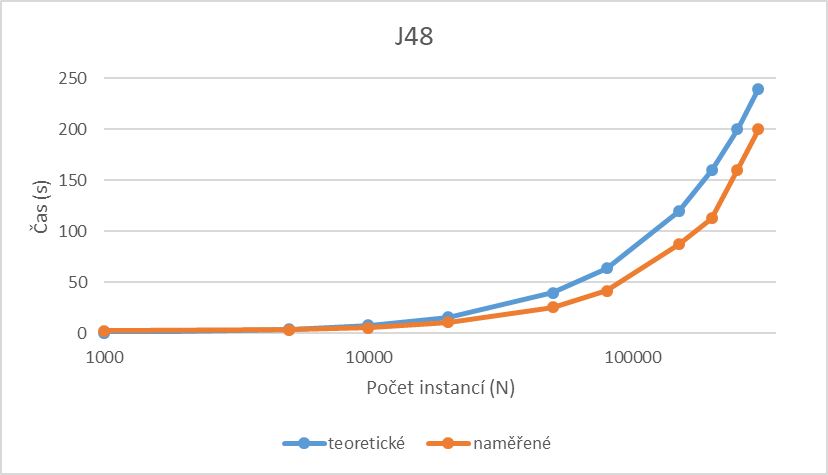
\includegraphics[scale=1]{img/j48.png}
  \caption{J48 - čas v závislosti na počtu instancí}
\end{figure}
\podsekce{Čas}
Teoretická časová složitost této implementace je $O(Nm^2)$ až $O(N^2)$ (pro numerické atributy a nevhodné rozložení dat). Z obrázku 7 lze vyčíst, že pro naše měření s nominálními atributy je složitost v lineární rovině. 

\newpage
\sekce{HoeffdingTree}
\paragraph{Charakter vstupních dat}
Vygenerovaná vstupní data jsou stejná jako pro J48. To mimo jiné umožňuje porovnání těchto algoritmů mezi sebou.
\paragraph{Nastavení algoritmu}
Parametr \textit{hoeffdingTieThreshold} nastaven na 0,05, \textit{gracePeriod}: 200.
\begin{figure}[hbp]
  \centering
  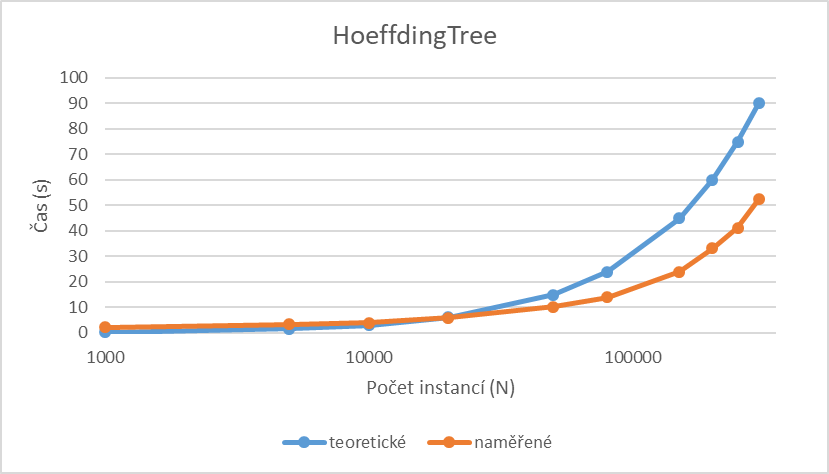
\includegraphics[scale=1]{img/ht.png}
  \caption{HoeffdingTree - čas v závislosti na počtu instancí}
\end{figure}
\podsekce{Čas}
Časová složitost je zde lineární, konkrétně $O(Nm)$, což je také vidět z~obrázku 8. Porovnání s algoritmem J48 následuje v kapitole 6.1.

\newpage
\sekce{JRip}
\paragraph{Charakter vstupních dat}
Soubor vstupních dat je opět shodný s datasety použitými pro NaiveBayes.
\paragraph{Nastavení algoritmu}
Parametr \textit{folds} (určuje množství dat pro prořezávání) nastaven na hodnotu 3, minimální celková váha instancí v pravidle \textit{minNo}: 2,0.
\begin{figure}[hbp]
  \centering
  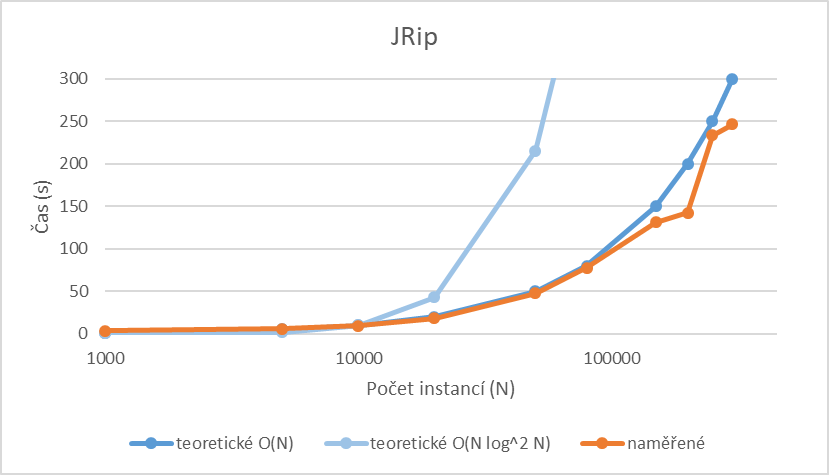
\includegraphics[scale=1]{img/jrip.png}
  \caption{JRip - čas v závislosti na počtu instancí}
\end{figure}
\podsekce{Čas}
Podle práce \textit{An Efficient Algorithm for Generating Classification Rules} je časová složitost algoritmu JRip $O(N log^2 N)$ \citep{vijay}. V obrázku 9 křivku této složitosti zobrazuje světle modrá barva. Ze získaných dat však můžeme vyvodit průměrnou složitost spíš jako lineární, $\Theta(N)$, jak také naznačuje tmavě modrá křivka.

\newpage
\sekce{LinearRegression}
\paragraph{Charakter vstupních dat}
Vytvoření vstupních datasetů proběhlo s generátorem MexicanHat. Parametr \textit{amplitude} byl ponechán na 1,0 a do datasetů nebyl přidáván žádný šum (\textit{noiseRate} = 0). Bylo vytvořeno 11 datasetů s počtem instancí od 1000 po 400000.
\paragraph{Nastavení algoritmu}
Parametry algoritmu byly ponechány na výchozích hodnotách Weky (\textit{attributeSelectionMethod}: M5 method, \textit{batchSize}: 100).
\begin{figure}[hbp]
  \centering
  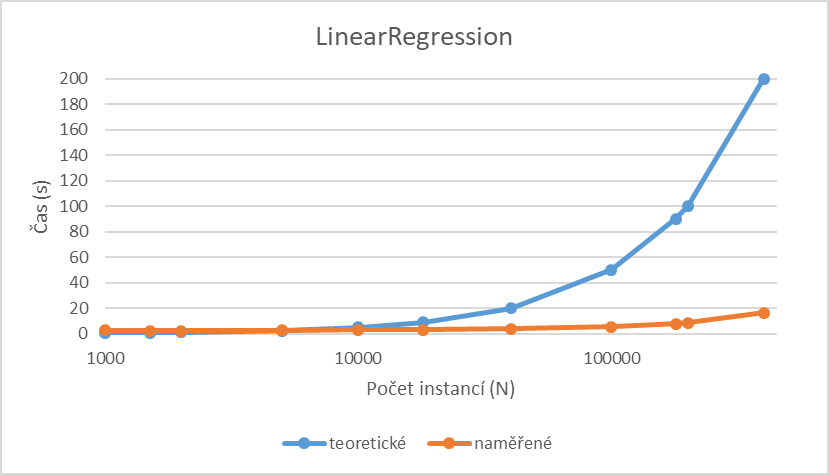
\includegraphics[scale=1]{img/linear.png}
  \caption{LinearRegression - čas v závislosti na počtu instancí}
\end{figure}
\podsekce{Čas}
Teoretická časová složitost algoritmu je lineární, $O(N)$. Algoritmus na umělých i reálných datasetech provedl svůj výpočet opravdu rychle, jak je i možné vidět v přiložených tabulkách. Z obrázku 10 se dá usoudit, že lineární teoretickou složitost má algoritmus opravdu jen pro nejhorší případy, průměrná časová složitost by nejspíš byla logaritmická. 

\newpage
\sekce{SimpleLogistic}
\paragraph{Charakter vstupních dat}
Zde byly použité datasety generovány pomocí RDG1 generátoru. Nastavení \textit{maxRuleSize}: 10, \textit{minRuleSize}: 1, \textit{numClasses}: 2. Počet atributů (\textit{numAttributes}) byl nastaven na 5. Bylo vytvořeno 11 datasetů s počtem instancí od 1000 po 300000.
\paragraph{Nastavení algoritmu}
Parametr \textit{heuristicStop} byl ponechán na 50, \textit{maxBoostingIterations}: 500.
\begin{figure}[hbp]
  \centering
  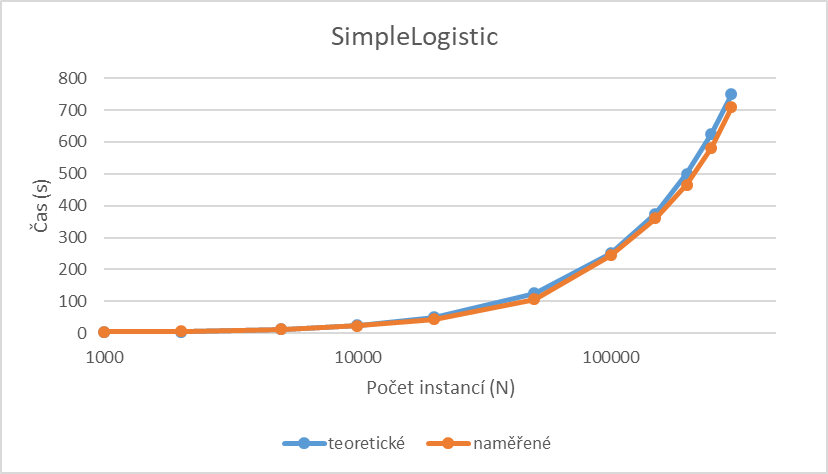
\includegraphics[scale=1]{img/logistic.png}
  \caption{SimpleLogistic - čas v závislosti na počtu instancí}
\end{figure}
\podsekce{Čas}
Na obrázku 11 vidíme, že teoretická křivka algoritmu je téměř identická s naměřenou. Zde je lineární časová složitost $O(N)$ velmi přesná.

\newpage
\sekce{SimpleKMeans}
\paragraph{Charakter vstupních dat}
Umělé datasety byly tvořeny BIRCHCluster generátorem. Počet shluků \textit{numClusters} nastaven na 2 a počet atributů \textit{numAttributes} nastaven na 30. Ostatní nastavení ponechána výchozí. Bylo vytvořeno 10 datasetů s počtem instancí od 1000 do 250000 rovnoměrně rozloženými mezi oba shluky.
\paragraph{Nastavení algoritmu}
Maximální počet iterací \textit{maxIterations} nastaven na 500, počet shluků \textit{numClusters}: 2 a počet vláken využitých pro běh algoritmu \textit{numExecutionSlots} na 1. Ostatní parametry ponechány výchozí.
\begin{figure}[hbp]
  \centering
  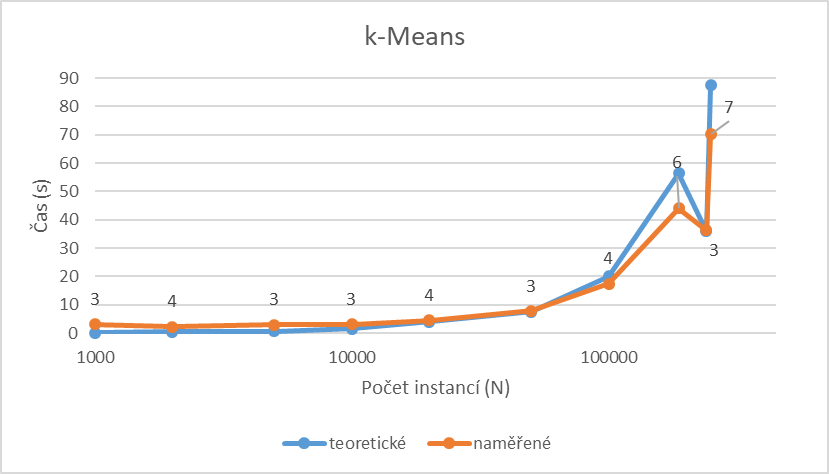
\includegraphics[scale=1]{img/kmeans.png}
  \caption{k-Means - čas v závislosti na počtu instancí}
\end{figure}
\podsekce{Čas}
Teoretická časová složitost tohoto algoritmu je $O(tkNm)$. Počet shluků je konstanta, počet atributů taktéž. Počet iterací potřebných pro konvergenci však nastavit nemůžeme, zanedbat také ne. Na obrázku 12 vidíme chování algoritmu v závislosti času na počtu instancí, zanedbáváme zde ovšem počet iterací, aby se dalo chování nějak zobrazit. Čísla u bodů v~grafu udávají počet potřebných iterací algoritmu. Z tohoto grafu bohužel nemůžeme vyvodit žádné závěry, kvůli třetí proměnné.
\podsekce{Paměť}
Horní hranice prostorové složitosti K-Means je opět lineární vzhledem k~$N$, a to $O((N+k)m)$. Z obrázku 13 můžeme usoudit, že očekávaná prostorová složitost je taktéž lineární. 
\begin{figure}[h]
  \centering
  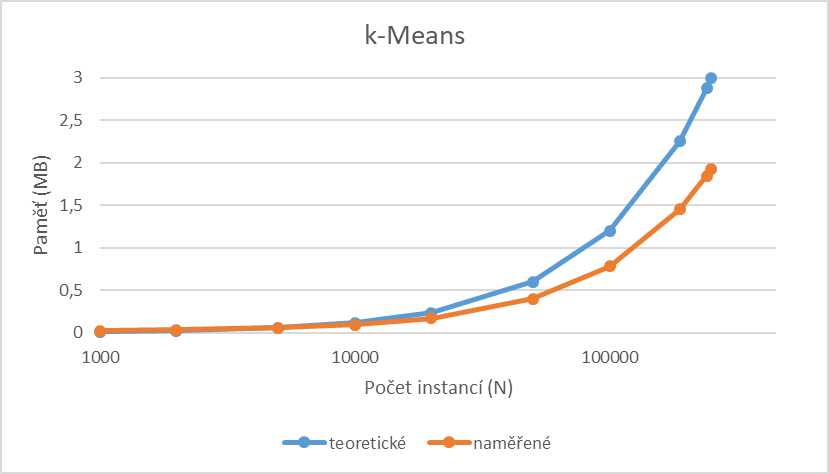
\includegraphics[scale=1]{img/kmeansp.png}
  \caption{k-Means - paměť v závislosti na počtu instancí}
\end{figure}

\newpage
\sekce{EM}
\paragraph{Charakter vstupních dat}
Za použití stejného generátoru a jeho nastavení jako u SimpleKMeans zde bylo vytvořeno 9 datasetů s 5 atributy a~počtem instancí od 1000 do 200000. Za účelem porovnání s algoritmem SimpleKMeans byl běh tohoto algoritmu také otestován na 10 datasetech s postupně se zvyšujícím počtem instancí a atributů. Srovnání s tímto algoritmem se nachází v kapitole 6.2.
\paragraph{Nastavení algoritmu}
Maximální počet iterací \textit{maxIterations} ponechán na 100, \textit{numFolds} je 10 a \textit{numKMeansRun} také 10.
\begin{figure}[hbp]
  \centering
  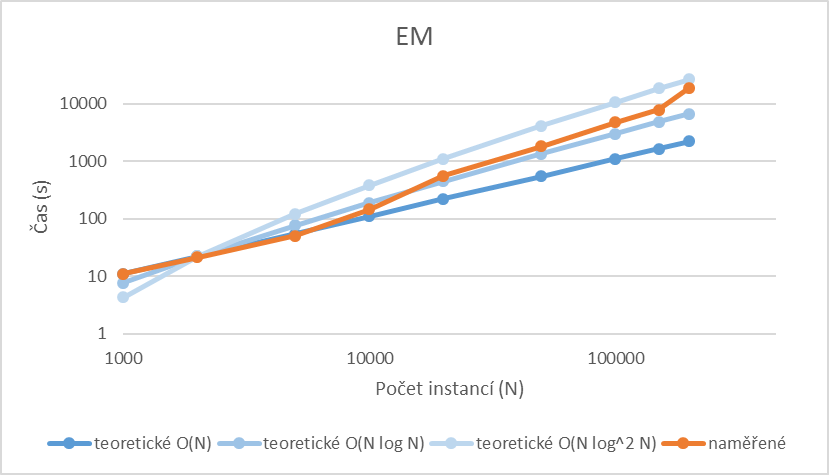
\includegraphics[scale=1]{img/em.png}
  \caption{EM - čas v závislosti na počtu instancí}
\end{figure}
\podsekce{Čas}
Časová složitost algoritmu je $O(Nmt)$ podle článku \textit{A Survey on Clustering Algorithms and Complexity Analysis}. \citep{uddin} 
\newline
\indent
Počet iterací algoritmu potřebných pro konvergenci byl na všech datasetech stejný (8). Na obrázku 14 je vidět chování algoritmu na syntetických datech a v odstínech modré barvy jsou pak zobrazeny teoretické křivky složitosti pro $O(N)$, $O(N log N)$ a $O(N log^2 N)$. Naměřené hodnoty zde překvapivě přesáhly předpokládanou lineární složitost a odpovídají spíš složitosti lineárně logaritmické.
\podsekce{Paměť}
Horní odhad prostorové složitosti algoritmu je stejný jako časové, tedy $O(Nmt)$. Obrázek 15 naznačuje, že tento odhad je přesný i pro očekávanou prostorovou složitost.
\begin{figure}[hbp]
  \centering
  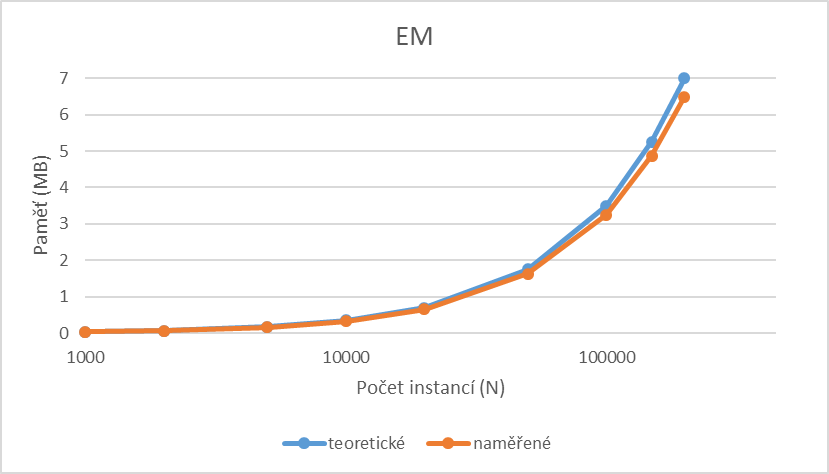
\includegraphics[scale=1]{img/emp.png}
  \caption{EM - paměť v závislosti na počtu instancí}
\end{figure}

\newpage
\sekce{IBk}
\paragraph{Charakter vstupních dat}
Pro testování na tomto algoritmu byly použity stejné datasety jako pro SimpleLogistic. Největší použitý dataset zde měl počet instancí 250000.
\paragraph{Nastavení algoritmu}
Počet sousedů \textit{KNN} nastaven na 1, jako \textit{nearestNeighbourSearchAlgorithm} byl ponechán LinearNNSearch.
\begin{figure}[hbp]
  \centering
  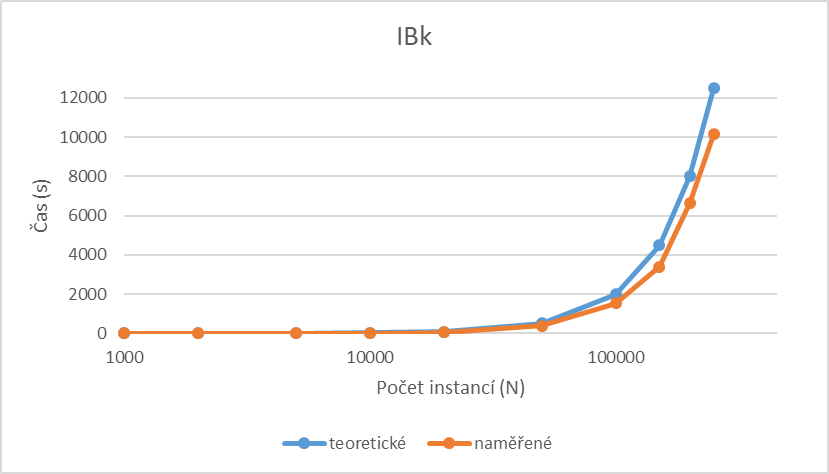
\includegraphics[scale=1]{img/ibk.png}
  \caption{IBk - čas v závislosti na počtu instancí}
\end{figure}
\podsekce{Čas}
Časová složitost je pro tento algoritmus kvadratická, $O(N^2)$. Na obrázku 16 vidíme, že tato složitost víceméně odpovídá i naměřeným hodnotám. Z tabulek si můžeme všimnout, že běh algoritmu na reálných datech byl podstatně rychlejší, než na datech syntetických.

\newpage
\sekce{SMO}
\paragraph{Charakter vstupních dat}
Tady bylo opět využito stejných datasetů jako v~případě SimpleLogistic.
\paragraph{Nastavení algoritmu}
Kalibrační metoda \textit{calibrator} zvolena jako Logistic, parametr složitosti \textit{c} ponechán na hodnotě 1.
\begin{figure}[hbp]
  \centering
  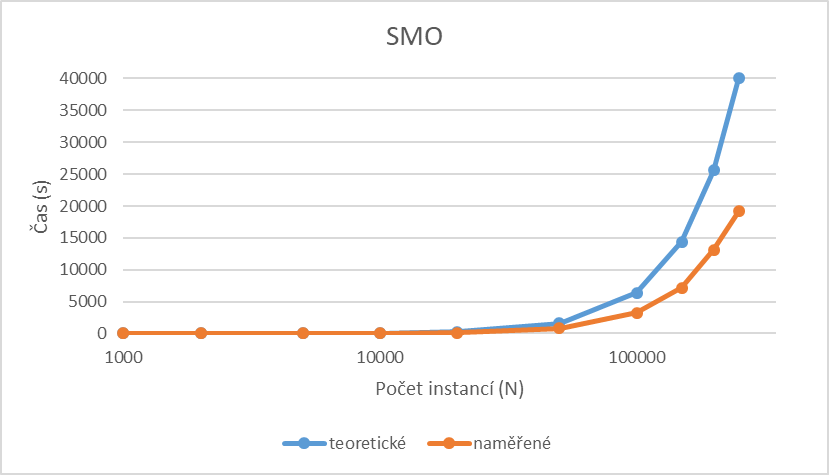
\includegraphics[scale=1]{img/smo.png}
  \caption{SMO - čas v závislosti na počtu instancí}
\end{figure}
\podsekce{Čas}
V nejhorších případech může mít tento algoritmus až kubickou časovou složitost $O(N^3)$. Na vygenerovaných datech se ovšem čas blížil kvadratické složitosti $O(N^2)$, jak je vidět z obrázku 17. V tabulkách jsou uvedeny i~výsledky testů pro postupně vyšší počet atributů i instancí, kde při 80 atributech a 100000 instancích převyšoval výpočet dobu běhu 52 hodin.
\newline
\indent
Pro zajímavost je na obrázku 18 zobrazena časová závislost algoritmu na počtu instancí na reálných datech v případě zanedbání počtu atributů.
\begin{figure}[hbp]
  \centering
  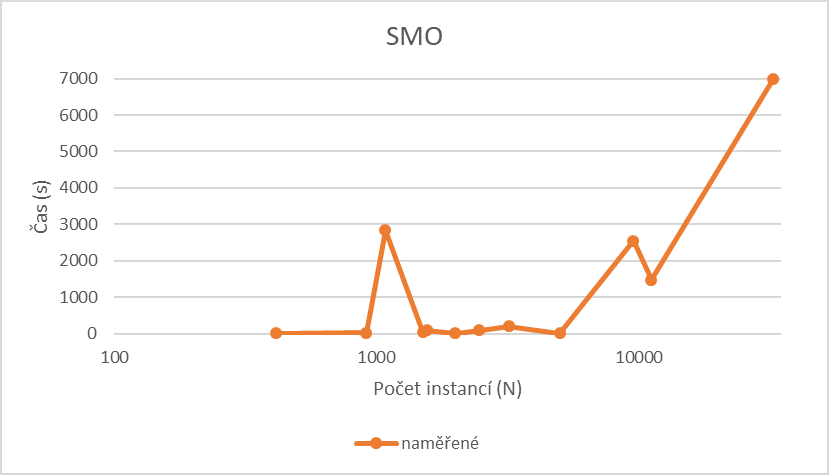
\includegraphics[scale=1]{img/smoreal.png}
  \caption{SMO - reálné datasety při zanedbání počtu atributů}
\end{figure}
\podsekce{Paměť}
Obrázek 19 znázorňuje teoretickou paměťovou složitost $O(N^2)$, ale na testovaných syntetických datech je tato složitost velmi nadsazena. Očekávaná paměťová složitost se zde pohybuje spíš v nižším řádu.
\begin{figure}[hbp]
  \centering
  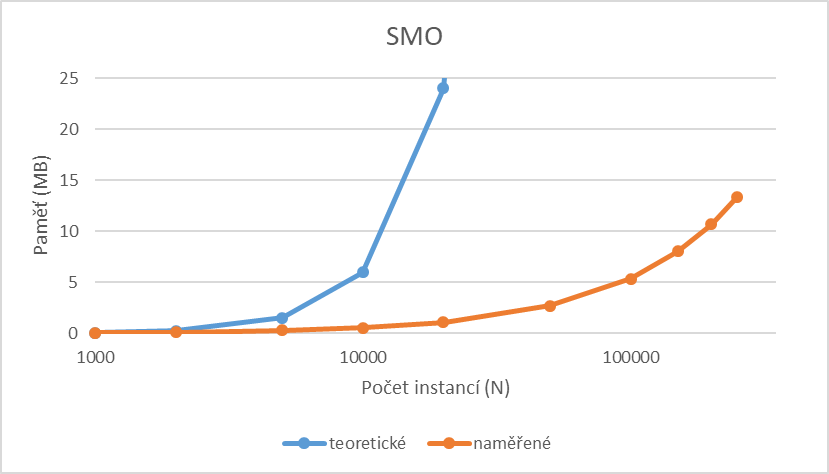
\includegraphics[scale=1]{img/smop.png}
  \caption{SMO - paměť v závislosti na počtu instancí}
\end{figure}

\newpage
\sekce{Apriori}
\paragraph{Charakter vstupních dat}
Pro tento algoritmus byla vytvořena data pomocí RDG1 generátoru. Nastavení \textit{maxRuleSize}: 10, \textit{minRuleSize}: 1, \textit{numClasses}: 2. Byly vytvořeny dvě skupiny datasetů po 11 s počtem instancí od 1000 po 300000. Pro první skupinu byl počet atributů (\textit{numAttributes}) nastaven na 5, pro druhou na 10.
\paragraph{Nastavení algoritmu}
Parametr udávající počet pravidel k nalezení \textit{numRules} byl nastaven na 10.
\begin{figure}[hbp]
  \centering
  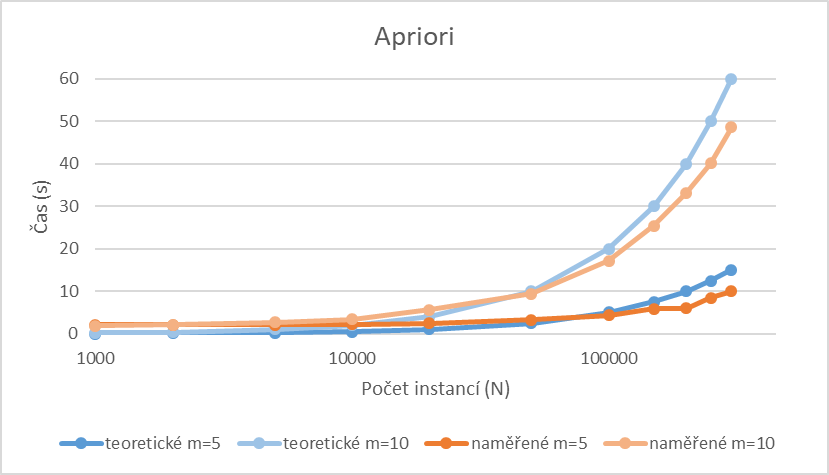
\includegraphics[scale=1]{img/apriori.png}
  \caption{Apriori - čas v závislosti na počtu instancí}
\end{figure}
\podsekce{Čas}
Teoretická časová složitost Apriori je $O(Nm)$ až $O(Nm^2)$. Na obrázku 20 je znázorněno chování pro datasety s počtem atributů $m=5$ i pro $m=10$. Očekávaná časová složitost je zde lineární vzhledem k počtu instancí, jestli je to ovšem $\Theta(Nm)$ nebo $\Theta(Nm^2)$ už nebylo podrobněji zkoumáno. Z~výsledků z tabulek pro datasety s různým počtem instancí i atributů se však dá usoudit, že je kvadratická vzhledem k počtu atributů.\footnote{Na datasetu se 100 atributy a 200000 instancemi byl naměřen průměrný čas 32 hodin, pro dataset s 80 atributy a polovičním počtem instancí trvala doba výpočtu pod dvě hodiny.} 

\kapitola{Porovnání a interpretace výsledků}
Tato práce je zaměřena na srovnání běhu vybraných algoritmů s jejich teoretickou složitostí, přesto se zde však nabízí možnost porovnat některé algoritmy mezi sebou. Klasifikační stromové algoritmy J48 a HoeffdingTree byly testovány na shodných vstupních datech a jejich srovnání se nachází v následující kapitole. Shlukovací algoritmy SimpleKMeans a~EM mají společné dvě skupiny vstupních dat a jejich chování na těchto datech je srovnáno v kapitole 6.2.

\newpage
\sekce{Porovnání rozhodovacích stromů}
V následujících grafech jsou zobrazeny výsledky testů pro srovnání J48 a HoeffdingTree. Při porovnání paměti potřebné k výpočtu na reálných i syntetických datech byla uvažována celková paměť využitá algoritmem (ne pouze velikost vytvořené struktury). To nám dává možnost úvahy pro volbu stroje s dostatečnou velikostí RAM.

\newpage
\podsekce{Reálné datasety}
Chování algoritmů na reálných datasetech nelze velmi dobře předvídat z~důvodu různorodosti charakteru datasetů. Algoritmus J48 běžel na datasetu \textit{new3s.wc} déle než 61 hodin a jeho běh musel být zastaven z časových důvodů.
\paragraph{Čas}
Obrázek 21 udává dobu běhu algoritmů na reálných datasetech. Kromě nejmenších vstupů je zde HoeffdingTree o něco rychlejší na všech reálných datasetech. Výpočet na největším vstupu \textit{new3s.wc} byl schopen provést v přijatelném čase (17 hodin), na rozdíl od J48.
\begin{figure}[hbp]
  \centering
  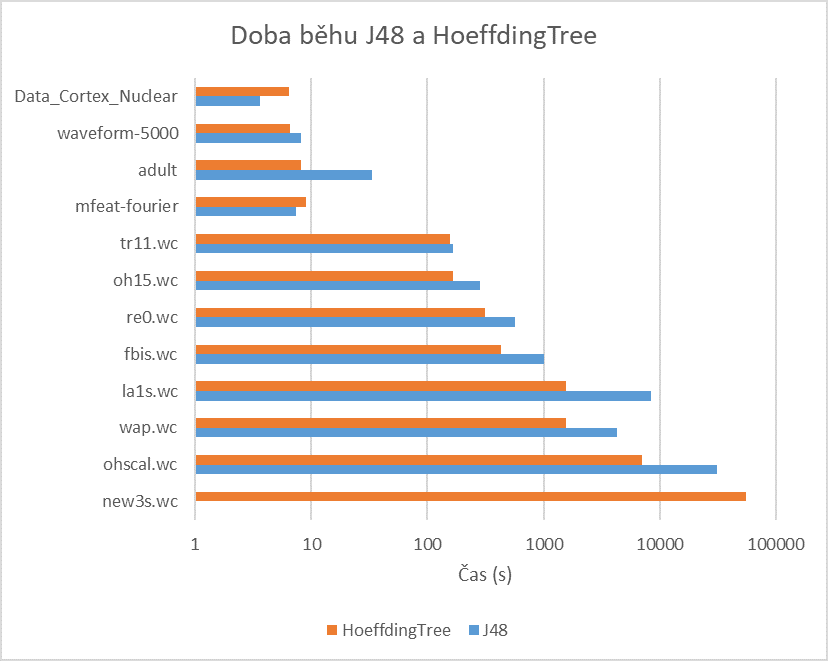
\includegraphics[scale=1]{img/realclasstime.png}
  \caption{Doba běhu J48 a HoeffdingTree na reálných datech}
\end{figure}

\newpage
\paragraph{Paměť}
Na obrázku 22 vidíme množství celkové paměti spotřebované oběma algoritmy pro svůj výpočet. V tomto případě vyniká pro změnu J48 na většině vstupů.
\begin{figure}[hbp]
  \centering
  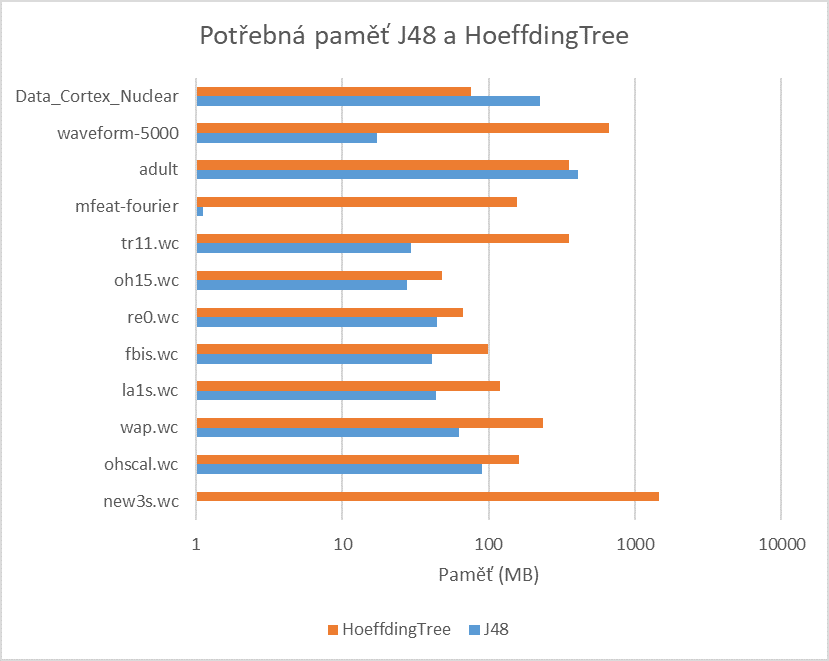
\includegraphics[scale=1]{img/realclassmem.png}
  \caption{Paměť J48 a HoeffdingTree na reálných datech}
\end{figure}

\newpage
\podsekce{Generované datasety}
Vygenerované datasety mají kromě počtu instancí a počtu atributů ostatní parametry totožné. Chování algoritmů na těchto vstupech je proto více předvídatelné. Datasety jsou pojmenovány podle počtu instancí a~atributů (např. \textit{1000-10-class} udává, že dataset obsahuje 1000 instancí po 10 atributech a je určen pro klasifikaci).
\paragraph{Čas}
Na obrázku 23 vidíme srovnání doby běhu algoritmů na vytvořených datasetech. HoeffdingTree je zde, stejně jako na reálných vstupech, rychlejší. S přibývající velikostí vstupu se rozdíl v čase zvyšuje.
\begin{figure}[hbp]
  \centering
  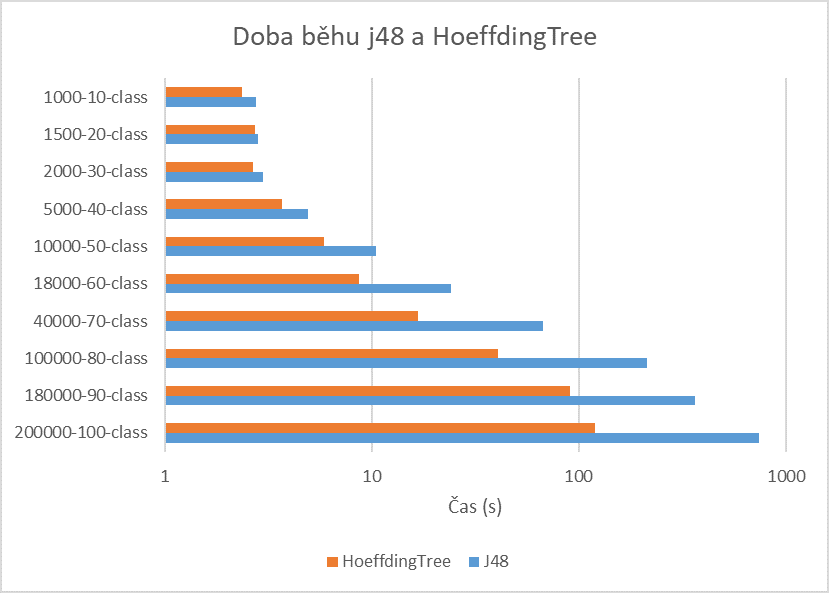
\includegraphics[scale=1]{img/genclasstime.png}
  \caption{Doba běhu J48 a HoeffdingTree na umělých datech}
\end{figure}

\newpage
\paragraph{Paměť}
Porovnání velikosti paměti potřebné k výpočtu je vidět na obrázku 24. Na tomto grafu je zajímavý fakt, že pro menší vstupy je k paměti šetrnější HoeffdingTree, na větších vstupech pak vítězí J48.
\begin{figure}[hbp]
  \centering
  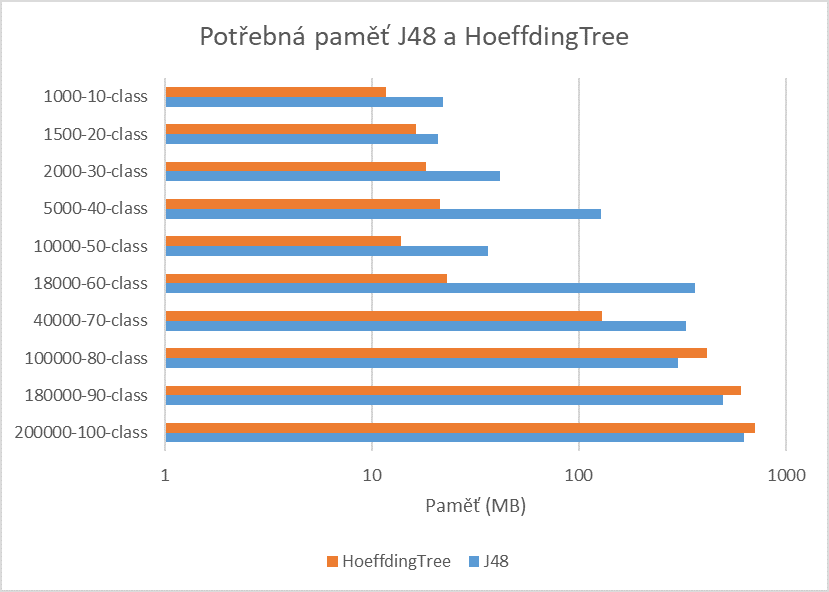
\includegraphics[scale=1]{img/genclassmem.png}
  \caption{Paměť J48 a HoeffdingTree na umělých datech}
\end{figure}

\newpage
\sekce{Porovnání shlukovacích algoritmů}
Tato kapitola obsahuje srovnání shlukovacích algoritmů SimpleKMeans a EM z hlediska času i paměti potřebné pro výpočet. Testování bylo provedeno na reálných i uměle vytvořených datech, stejně jako v případě rozhodovacích stromů. Počet iterací algoritmů byl omezen na 100, počet možných nalezených shluků nebyl nijak omezen.

\newpage
\podsekce{Reálné datasety}
Doba běhu algoritmu EM přesahovala na největších vstupech 61 hodin, proto byl jeho běh z časových důvodů zastaven. 
\paragraph{Čas}
Z obrázku 25 je jasně vidět, že jednoduchý SimpleKMeans má řádově nižší dobu běhu pro všechny zvolené reálné datasety. Z přiložených tabulek je také zajímavé zjištění, že počet iterací EM pro nejmenší vstupy dosahuje nastaveného maxima.
\begin{figure}[hbp]
  \centering
  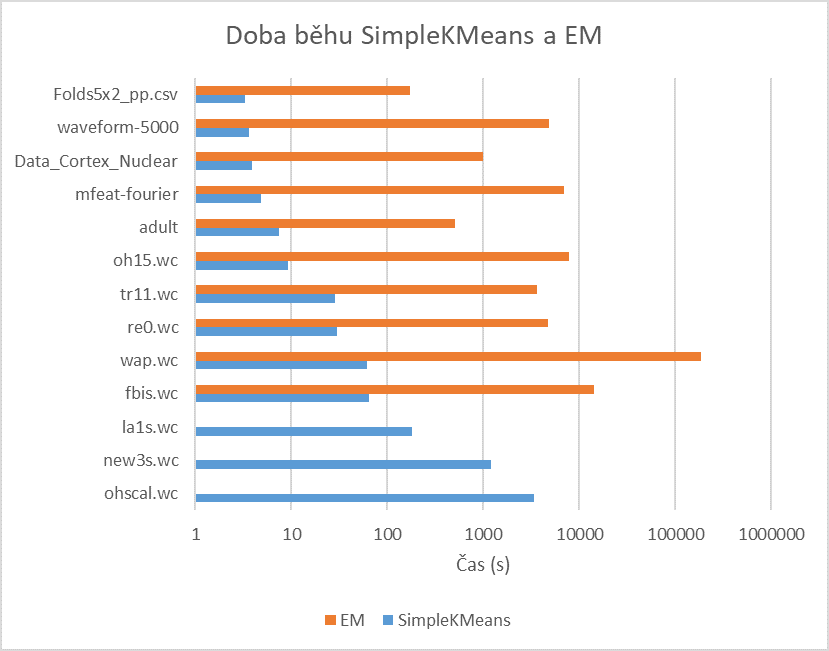
\includegraphics[scale=1]{img/realclusttime.png}
  \caption{Čas SimpleKMeans a EM na reálných datech}
\end{figure}

\newpage
\paragraph{Paměť}
Paměť potřebná k výpočtu je zde opět obecně vyšší pro EM, nejsou zde však tak znatelné rozdíly jako v případě doby běhu, jak vyplývá z obrázku 26.
\begin{figure}[hbp]
  \centering
  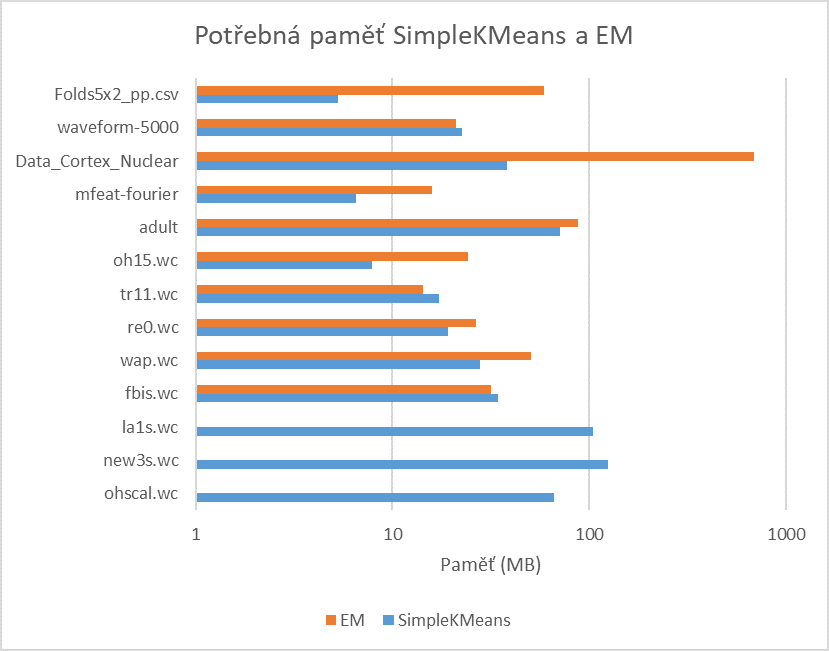
\includegraphics[scale=1]{img/realclustmem.png}
  \caption{Paměť SimpleKMeans a EM na reálných datech}
\end{figure}

\newpage
\podsekce{Generované datasety}
Algoritmus EM musel být na největších datasetech opět předčasně zastaven. Na uměle vytvořených datech si v tabulkách můžeme všimnout, že počet vytvořených shluků u EM je pro většinu zkoumaných datasetů dvojnásobný.
\paragraph{Čas}
Stejně jako v případě reálných vstupů je algoritmus SimpleKMeans na generovaných vstupech řádově rychlejší než EM (i přes vyšší počet iterací), jak je zobrazeno na obrázku 27. 
\begin{figure}[hbp]
  \centering
  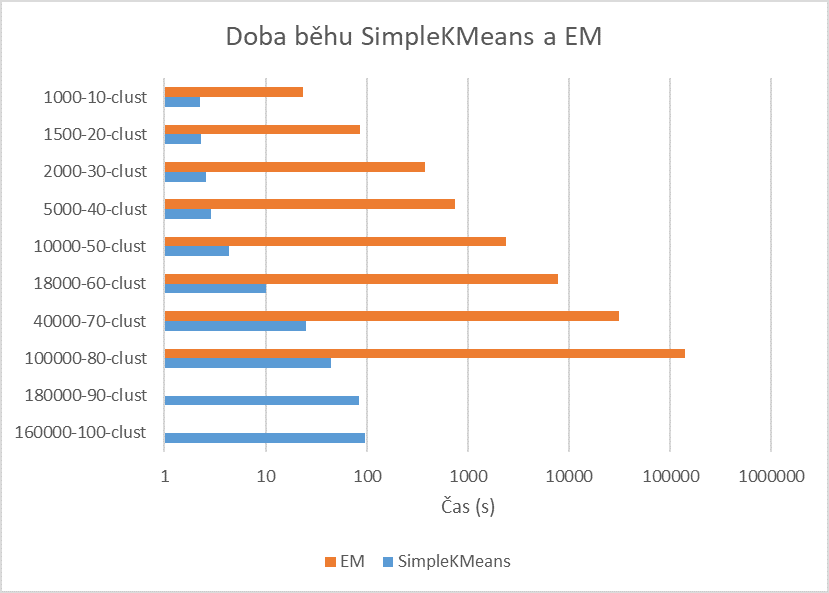
\includegraphics[scale=1]{img/genclusttime.png}
  \caption{Čas SimpleKMeans a EM na umělých datech}
\end{figure}

\newpage
\paragraph{Paměť}
Obrázek 28 poukazuje na překvapivé zjištění, že pro větší vstupy je EM z hlediska paměti lepší, než SimpleKMeans.
\begin{figure}[hbp]
  \centering
  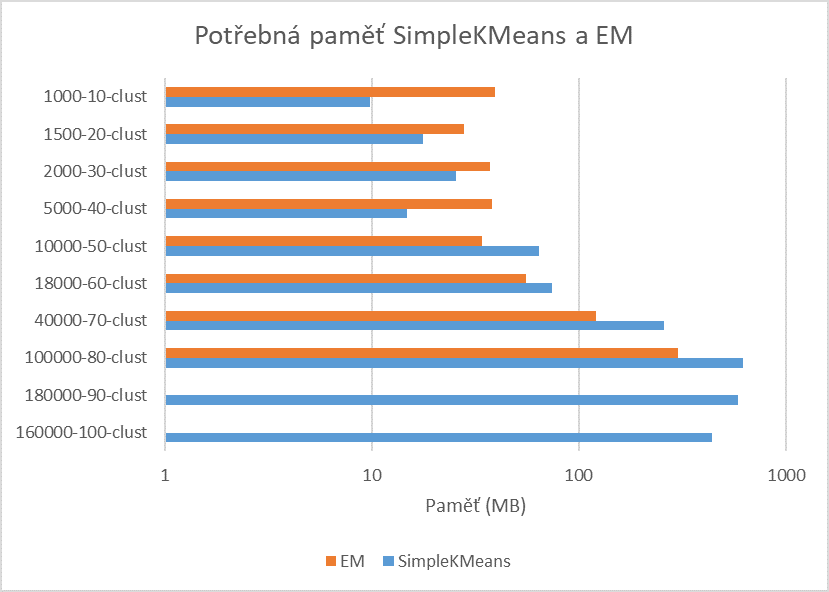
\includegraphics[scale=1]{img/genclustmem.png}
  \caption{Paměť SimpleKMeans a EM na umělých datech}
\end{figure}


\kapitola{Diskuze}
\sekce{Platnost výsledků}
Naměřené hodnoty algoritmů je třeba chápat v souvislosti se zvolenou metodikou. Pokud bychom využili pro testování jiné prostředí než Java a~JVM, nebo bychom zvolili jiné implementace algoritmů než Weka a jdmp, výsledky by zcela jistě byly rozdílné. Dále je nutné poznamenat, že  na ovlivnění výsledků se také podílí využitý hardware. Zvlášť v případě JVM, kdy je alokace paměti pro výpočet zcela ponechána na virtuálním stroji (jak je popsáno v kapitole 4.2.2), hraje velkou roli velikost dostupné operační paměti RAM a její frekvence. Doba běhu algoritmu samozřejmě závisí především na výkonu procesoru. Lepší čas výpočtu můžeme také získat implementací paralelního zpracování, využitím více vláken i více jader procesoru. Teoretická složitost algoritmů by ale hardwarem být ovlivněna neměla. 

\sekce{Doporučení}
Volba algoritmu záleží především na tom, jakou úlohu chceme na vstupních datech provádět. Některé algoritmy také pracují jen s nominálními atributy, jiné i s numerickými. Volba algoritmu taktéž záleží na tom, zda-li pro danou úlohu upřednostňujeme přesnost, nižší dobu výpočtu a nebo nižší velikost potřebné paměti. Ve většině případů je nejdůležitější doba výpočtu spolu s přesností. Problém velikosti potřebné paměti lze v dnešní době částečně vyřešit přidáváním RAM paměti do výpočetního stroje.
\newline
\indent
Z výsledků důslednějšího srovnání klasifikačních algoritmů J48 a~HoeffdingTree lze doporučit HoeffdingTree, stejně jako ve své práci zdůrazňuje Desai. \citep{desai} 
\newline
\indent
V širším spektru pak lze v úloze klasifikace vyzdvihnout algoritmus NaiveBayes jak z hlediska doby běhu, tak z hlediska paměti a relativní přesnosti na testovaných datech. Algoritmus IBk také můžeme zařadit jako vhodnou volbu v případě omezené operační paměti. Algoritmus SMO, jak už napovídá odhad teoretické složitosti (může být až $O(N^3)$), se v provedených testech zařadil mezi nejpomalejší algoritmy (na některých generovaných datasetech musel být běh po 60 hodinách zastaven) s relativně velkou paměťovou náročností, proto by měl být volen spíš pro specifické úlohy, kde nelze použít lineární verzi tohoto algoritmu a nezáleží na rychlosti běhu. Na testovaných datech ovšem prokazoval velmi dobrou přesnost klasifikace (spolu s algoritmem JRip).
\newline
\indent
Srovnání obou vybraných shlukovacích algoritmů naznačuje, že SimpleKMeans je mnohem rychlejší než EM na všech testovaných datech. Výběr algoritmu EM lze uvážit v případě běhu na velkých datasetech a~omezeném množství operační paměti. V tomto případě by ovšem bylo nejspíš vhodnější vyhledat jiný algoritmus pro tento typ úlohy.
\newline
\indent
Volba algoritmu pro regresní analýzu záleží na tom, jestli chceme provádět lineární nebo logistickou regresi. Oba testované algoritmy vykazovaly velmi dobrou rychlost výpočtu. U SimpleLogistic však musíme počítat s vyšší potřebou zabrané paměti.
\newline
\indent
V úloze hledání asociačních pravidel byl testován pouze algoritmus Apriori. Pro opodstatnění výběru tohoto algoritmu by bylo potřebné vyzkoušet další algoritmy vhodné pro tuto úlohu. 

\kapitola{Závěr}
Práce nabízí podrobné srovnání 11 nejběžnějších algoritmů používaných v oboru data mining. V teoretické části práce byly popsány jednotlivé algoritmy a zdůvodněn jejich výběr. Důraz byl kladen na výběr algoritmů pro co největší množství typů úloh. Dále byla zjištěna teoretická složitost každého algoritmu a podrobně rozepsána problematika algoritmické složitosti. Následně byly vybrány vhodné datasety. Zde byl brán důraz na vyhledání reálných datasetů s co největší velikostí. Zde narážíme na problém týkající se dostupného množství informací o veřejných datasetech. Tento problém je podrobněji popsán v kapitole 2.5. 
\newline
\indent
Díky programu Weka (a knihovny jdmp) odpadl problém hledání konkrétních implementací jednotlivých algoritmů. Weka má i api pro Javu, což z ní učinilo nejvhodnější nástroj pro řešení praktické části této práce. Pomocí rozhraní Weky a vhodným využitím metod Javy pro zjištění času i~paměti potřebné pro běh algoritmů byly otestovány všechny algoritmy na syntetických i reálných datech. Zpočátku bylo vybráno více algoritmů, ale průběžné testy ukázaly, že některé algoritmy z hlediska své vysoké paměťové nebo časové složitosti nejsou vhodné pro další testování v rámci této práce.  
\newline
\indent
Hlavním cílem práce nebylo získat nějaké překvapivé výsledky nebo objevit přelomové znalosti, ale spíš porovnat reálné chování algoritmů s jejich teoretickými předpoklady. Z těchto výsledků je pak možné orientačně určit vhodný algoritmus pro novou úlohu bez nutnosti časově náročného zkoušení více potenciálních kandidátů a nebo náhodného výběru. 
\newline
\indent
Rozdíly mezi některými algoritmy data miningu v náročnosti na čas a~prostor byly nemalé. U většiny případů se potvrdila souvislost s teoretickou složitostí podle notace velké $O$. V kapitole 5 můžeme nalézt i odhad průměrné složitosti algoritmů. Pro eliminaci náhodných vlivů na hodnoty měření byl každý algoritmus spuštěn minimálně pětkrát pro každý vstup.
\newline
\indent
Praktická část práce popisuje metodiku zvolenou pro způsob testování a porovnání algoritmů. Nastiňuje také problémy s nalezením teoretických složitostí konkrétních implementací a srozumitelným zobrazením výsledků. 
\newline
\indent
V kapitole 5 jsou pak vhodně graficky znázorněny naměřené výsledky a orientační porovnání algoritmů s jejich teoretickými složitostmi. Přesné výsledky měření na dalších skupinách vstupů spolu s doplňujícími informacemi (přesnost klasifikace, nalezený počet shluků, pravidel atd.) jsou pak dostupné v tabulkách na přiloženém CD. Některé výsledky byly ovšem překvapivé. Například průměrná složitost lineární regrese z testů vychází mnohem lépe, než je její horní odhad složitosti. Naproti tomu shlukovací algoritmus EM vykazoval na testovaných datech vyšší složitost, než je udávaný horní odhad.
\newline
\indent
Doporučený výběr algoritmů pro konkrétní typy úloh je uveden v kapitole 6. Můžeme zde vyzdvihnout algoritmy NaiveBayes a SimpleKMeans jakožto nejvhodnější testované algoritmy pro řešení úloh klasifikace a shlukování s ohledem na přijatelnou paměťovou náročnost.
\newline
\indent
V kapitole 4.1.1 je uveden problém nalezení horního odhadu prostorové složitosti u různých algoritmů a jejich implementací. Jako rozšíření této práce by byl jistě zajímavý úkol hledání dosud neznámých složitostí nejčastějších algoritmů pro data mining. 
\newline
\indent
Závěrem lze říci, že tato práce přinesla využitelné hmatatelné výsledky a byl splněn cíl práce, který byl kladený na začátku.
\bibliographystyle{apalike}
\bibliography{bibliography}
\prilohy
\kapitola{CD}
\paragraph{Obsah}
\begin{enumerate}
\item Zdrojové kódy všech skriptů
\item Všechny použité datasety
\item Tabulky s výsledky, grafy a informacemi o datasetech
\item Samotná práce ve formátu LaTex i PDF
\end{enumerate}

\end{document}

